% Options for packages loaded elsewhere
\PassOptionsToPackage{unicode}{hyperref}
\PassOptionsToPackage{hyphens}{url}
%
\documentclass[
]{article}
\usepackage{amsmath,amssymb}
\usepackage{iftex}
\ifPDFTeX
  \usepackage[T1]{fontenc}
  \usepackage[utf8]{inputenc}
  \usepackage{textcomp} % provide euro and other symbols
\else % if luatex or xetex
  \usepackage{unicode-math} % this also loads fontspec
  \defaultfontfeatures{Scale=MatchLowercase}
  \defaultfontfeatures[\rmfamily]{Ligatures=TeX,Scale=1}
\fi
\usepackage{lmodern}
\ifPDFTeX\else
  % xetex/luatex font selection
\fi
% Use upquote if available, for straight quotes in verbatim environments
\IfFileExists{upquote.sty}{\usepackage{upquote}}{}
\IfFileExists{microtype.sty}{% use microtype if available
  \usepackage[]{microtype}
  \UseMicrotypeSet[protrusion]{basicmath} % disable protrusion for tt fonts
}{}
\makeatletter
\@ifundefined{KOMAClassName}{% if non-KOMA class
  \IfFileExists{parskip.sty}{%
    \usepackage{parskip}
  }{% else
    \setlength{\parindent}{0pt}
    \setlength{\parskip}{6pt plus 2pt minus 1pt}}
}{% if KOMA class
  \KOMAoptions{parskip=half}}
\makeatother
\usepackage{xcolor}
\usepackage[margin=1in]{geometry}
\usepackage{color}
\usepackage{fancyvrb}
\newcommand{\VerbBar}{|}
\newcommand{\VERB}{\Verb[commandchars=\\\{\}]}
\DefineVerbatimEnvironment{Highlighting}{Verbatim}{commandchars=\\\{\}}
% Add ',fontsize=\small' for more characters per line
\usepackage{framed}
\definecolor{shadecolor}{RGB}{248,248,248}
\newenvironment{Shaded}{\begin{snugshade}}{\end{snugshade}}
\newcommand{\AlertTok}[1]{\textcolor[rgb]{0.94,0.16,0.16}{#1}}
\newcommand{\AnnotationTok}[1]{\textcolor[rgb]{0.56,0.35,0.01}{\textbf{\textit{#1}}}}
\newcommand{\AttributeTok}[1]{\textcolor[rgb]{0.13,0.29,0.53}{#1}}
\newcommand{\BaseNTok}[1]{\textcolor[rgb]{0.00,0.00,0.81}{#1}}
\newcommand{\BuiltInTok}[1]{#1}
\newcommand{\CharTok}[1]{\textcolor[rgb]{0.31,0.60,0.02}{#1}}
\newcommand{\CommentTok}[1]{\textcolor[rgb]{0.56,0.35,0.01}{\textit{#1}}}
\newcommand{\CommentVarTok}[1]{\textcolor[rgb]{0.56,0.35,0.01}{\textbf{\textit{#1}}}}
\newcommand{\ConstantTok}[1]{\textcolor[rgb]{0.56,0.35,0.01}{#1}}
\newcommand{\ControlFlowTok}[1]{\textcolor[rgb]{0.13,0.29,0.53}{\textbf{#1}}}
\newcommand{\DataTypeTok}[1]{\textcolor[rgb]{0.13,0.29,0.53}{#1}}
\newcommand{\DecValTok}[1]{\textcolor[rgb]{0.00,0.00,0.81}{#1}}
\newcommand{\DocumentationTok}[1]{\textcolor[rgb]{0.56,0.35,0.01}{\textbf{\textit{#1}}}}
\newcommand{\ErrorTok}[1]{\textcolor[rgb]{0.64,0.00,0.00}{\textbf{#1}}}
\newcommand{\ExtensionTok}[1]{#1}
\newcommand{\FloatTok}[1]{\textcolor[rgb]{0.00,0.00,0.81}{#1}}
\newcommand{\FunctionTok}[1]{\textcolor[rgb]{0.13,0.29,0.53}{\textbf{#1}}}
\newcommand{\ImportTok}[1]{#1}
\newcommand{\InformationTok}[1]{\textcolor[rgb]{0.56,0.35,0.01}{\textbf{\textit{#1}}}}
\newcommand{\KeywordTok}[1]{\textcolor[rgb]{0.13,0.29,0.53}{\textbf{#1}}}
\newcommand{\NormalTok}[1]{#1}
\newcommand{\OperatorTok}[1]{\textcolor[rgb]{0.81,0.36,0.00}{\textbf{#1}}}
\newcommand{\OtherTok}[1]{\textcolor[rgb]{0.56,0.35,0.01}{#1}}
\newcommand{\PreprocessorTok}[1]{\textcolor[rgb]{0.56,0.35,0.01}{\textit{#1}}}
\newcommand{\RegionMarkerTok}[1]{#1}
\newcommand{\SpecialCharTok}[1]{\textcolor[rgb]{0.81,0.36,0.00}{\textbf{#1}}}
\newcommand{\SpecialStringTok}[1]{\textcolor[rgb]{0.31,0.60,0.02}{#1}}
\newcommand{\StringTok}[1]{\textcolor[rgb]{0.31,0.60,0.02}{#1}}
\newcommand{\VariableTok}[1]{\textcolor[rgb]{0.00,0.00,0.00}{#1}}
\newcommand{\VerbatimStringTok}[1]{\textcolor[rgb]{0.31,0.60,0.02}{#1}}
\newcommand{\WarningTok}[1]{\textcolor[rgb]{0.56,0.35,0.01}{\textbf{\textit{#1}}}}
\usepackage{graphicx}
\makeatletter
\def\maxwidth{\ifdim\Gin@nat@width>\linewidth\linewidth\else\Gin@nat@width\fi}
\def\maxheight{\ifdim\Gin@nat@height>\textheight\textheight\else\Gin@nat@height\fi}
\makeatother
% Scale images if necessary, so that they will not overflow the page
% margins by default, and it is still possible to overwrite the defaults
% using explicit options in \includegraphics[width, height, ...]{}
\setkeys{Gin}{width=\maxwidth,height=\maxheight,keepaspectratio}
% Set default figure placement to htbp
\makeatletter
\def\fps@figure{htbp}
\makeatother
\setlength{\emergencystretch}{3em} % prevent overfull lines
\providecommand{\tightlist}{%
  \setlength{\itemsep}{0pt}\setlength{\parskip}{0pt}}
\setcounter{secnumdepth}{5}
\ifLuaTeX
  \usepackage{selnolig}  % disable illegal ligatures
\fi
\IfFileExists{bookmark.sty}{\usepackage{bookmark}}{\usepackage{hyperref}}
\IfFileExists{xurl.sty}{\usepackage{xurl}}{} % add URL line breaks if available
\urlstyle{same}
\hypersetup{
  pdftitle={Statistical Inference and Modelling: Assignment 2},
  pdfauthor={Gabriel Vayá, Arnau Torru, Darryl Abraham},
  hidelinks,
  pdfcreator={LaTeX via pandoc}}

\title{Statistical Inference and Modelling: Assignment 2}
\author{Gabriel Vayá, Arnau Torru, Darryl Abraham}
\date{2023-12-13}

\begin{document}
\maketitle

{
\setcounter{tocdepth}{3}
\tableofcontents
}
\begin{Shaded}
\begin{Highlighting}[]
\CommentTok{\# Clear plots}
\ControlFlowTok{if}\NormalTok{(}\SpecialCharTok{!}\FunctionTok{is.null}\NormalTok{(}\FunctionTok{dev.list}\NormalTok{())) }\FunctionTok{dev.off}\NormalTok{()}
\end{Highlighting}
\end{Shaded}

\begin{verbatim}
## null device 
##           1
\end{verbatim}

\begin{Shaded}
\begin{Highlighting}[]
\CommentTok{\# Clean workspace}
\FunctionTok{rm}\NormalTok{(}\AttributeTok{list=}\FunctionTok{ls}\NormalTok{())}

\FunctionTok{library}\NormalTok{(car)}
\end{Highlighting}
\end{Shaded}

\begin{verbatim}
## Loading required package: carData
\end{verbatim}

\begin{Shaded}
\begin{Highlighting}[]
\FunctionTok{library}\NormalTok{(MASS)}
\FunctionTok{library}\NormalTok{(missMDA)}
\FunctionTok{library}\NormalTok{(visdat)}
\FunctionTok{library}\NormalTok{(FactoMineR)}
\FunctionTok{library}\NormalTok{(chemometrics)}
\end{Highlighting}
\end{Shaded}

\begin{verbatim}
## Loading required package: rpart
\end{verbatim}

\begin{Shaded}
\begin{Highlighting}[]
\FunctionTok{library}\NormalTok{(corrplot)}
\end{Highlighting}
\end{Shaded}

\begin{verbatim}
## corrplot 0.92 loaded
\end{verbatim}

\begin{Shaded}
\begin{Highlighting}[]
\FunctionTok{library}\NormalTok{(naniar)}
\FunctionTok{library}\NormalTok{(nortest)}
\FunctionTok{library}\NormalTok{(visdat)}
\FunctionTok{library}\NormalTok{(tidyverse)}
\end{Highlighting}
\end{Shaded}

\begin{verbatim}
## -- Attaching core tidyverse packages ------------------------ tidyverse 2.0.0 --
## v dplyr     1.1.4     v readr     2.1.4
## v forcats   1.0.0     v stringr   1.5.1
## v ggplot2   3.4.4     v tibble    3.2.1
## v lubridate 1.9.3     v tidyr     1.3.0
## v purrr     1.0.2
\end{verbatim}

\begin{verbatim}
## -- Conflicts ------------------------------------------ tidyverse_conflicts() --
## x dplyr::filter() masks stats::filter()
## x dplyr::lag()    masks stats::lag()
## x dplyr::recode() masks car::recode()
## x dplyr::select() masks MASS::select()
## x purrr::some()   masks car::some()
## i Use the conflicted package (<http://conflicted.r-lib.org/>) to force all conflicts to become errors
\end{verbatim}

\begin{Shaded}
\begin{Highlighting}[]
\FunctionTok{library}\NormalTok{(lsr)}
\FunctionTok{library}\NormalTok{(effects)}
\end{Highlighting}
\end{Shaded}

\begin{verbatim}
## lattice theme set by effectsTheme()
## See ?effectsTheme for details.
\end{verbatim}

First thing will be to load the data into R, and redeclaring the
variables to properly comply with the needs of the analysis. Notice we
relable the levels of the variable SeniorCitizen from (0,1) to (No, Yes)
for practical reasons.

\begin{Shaded}
\begin{Highlighting}[]
\CommentTok{\#setwd("C:\textbackslash{}\textbackslash{}Users\textbackslash{}\textbackslash{}darry\textbackslash{}\textbackslash{}Documents\textbackslash{}\textbackslash{}MDS\textbackslash{}\textbackslash{}Statistical\_Inference\_And\_Modelling\textbackslash{}\textbackslash{}SIM\_Assignment2")}
\CommentTok{\#setwd("/Users/gabrielvayaabad/Desktop/MDS/SIM/Assignment 2")}
\CommentTok{\#setwd("C:/Users/Admin/Desktop/MÀSTER DATA SCIENCE/SIM/Assigment 2")}
\FunctionTok{setwd}\NormalTok{(}\StringTok{"D:/MDS/ADSDB/SIM\_Assignment2"}\NormalTok{)}

\NormalTok{df }\OtherTok{\textless{}{-}} \FunctionTok{read.csv}\NormalTok{(}\StringTok{"WA\_Fn{-}UseC\_{-}Telco{-}Customer{-}Churn.csv"}\NormalTok{)}
\CommentTok{\#df \textless{}{-} WA\_Fn\_UseC\_Telco\_Customer\_Churn}

\NormalTok{df}\SpecialCharTok{$}\NormalTok{MonthlyCharges }\OtherTok{\textless{}{-}} \FunctionTok{as.numeric}\NormalTok{(df}\SpecialCharTok{$}\NormalTok{MonthlyCharges)}
\NormalTok{df}\SpecialCharTok{$}\NormalTok{TotalCharges }\OtherTok{\textless{}{-}} \FunctionTok{as.numeric}\NormalTok{(df}\SpecialCharTok{$}\NormalTok{TotalCharges)}
\NormalTok{df[}\FunctionTok{sapply}\NormalTok{(df, is.character)] }\OtherTok{\textless{}{-}} \FunctionTok{lapply}\NormalTok{(df[}\FunctionTok{sapply}\NormalTok{(df, is.character)], as.factor)}
\NormalTok{df}\SpecialCharTok{$}\NormalTok{SeniorCitizen }\OtherTok{\textless{}{-}} \FunctionTok{as.factor}\NormalTok{(df}\SpecialCharTok{$}\NormalTok{SeniorCitizen)}
\NormalTok{df}\SpecialCharTok{$}\NormalTok{customerID }\OtherTok{\textless{}{-}} \FunctionTok{as.character}\NormalTok{(df}\SpecialCharTok{$}\NormalTok{customerID)}
\FunctionTok{levels}\NormalTok{(df}\SpecialCharTok{$}\NormalTok{SeniorCitizen) }\OtherTok{\textless{}{-}} \FunctionTok{c}\NormalTok{(}\StringTok{"No"}\NormalTok{,}\StringTok{"Yes"}\NormalTok{)}
\end{Highlighting}
\end{Shaded}

\hypertarget{datapreparation}{%
\section{DataPreparation}\label{datapreparation}}

\hypertarget{missing-values}{%
\section{Missing Values}\label{missing-values}}

For the missing data, we see that there are only 11 missing values. If
we look even closer, we can see they are all in the same variable,
TotalCharges. Analysing even further, we can see those missing values
are corresponding to those clients with 0 month of tenure. Hence are
imputing them with 0.

\begin{Shaded}
\begin{Highlighting}[]
\FunctionTok{vis\_miss}\NormalTok{(df)}
\end{Highlighting}
\end{Shaded}

\includegraphics{Assignment2_script_files/figure-latex/unnamed-chunk-3-1.pdf}

\begin{Shaded}
\begin{Highlighting}[]
\CommentTok{\#df[is.na(df$TotalCharges),] \#NAs only found in TotalCharges variable}

\FunctionTok{mcar\_test}\NormalTok{(df) }\CommentTok{\#p{-}value is 0 {-}\textgreater{} not random}
\end{Highlighting}
\end{Shaded}

\begin{verbatim}
## # A tibble: 1 x 4
##   statistic    df p.value missing.patterns
##       <dbl> <dbl>   <dbl>            <int>
## 1      184.    20       0                2
\end{verbatim}

\begin{Shaded}
\begin{Highlighting}[]
\NormalTok{df}\SpecialCharTok{$}\NormalTok{tenure[}\FunctionTok{is.na}\NormalTok{(df}\SpecialCharTok{$}\NormalTok{TotalCharges)] }\CommentTok{\#TotalCharges are NA when tenure is 0}
\end{Highlighting}
\end{Shaded}

\begin{verbatim}
##  [1] 0 0 0 0 0 0 0 0 0 0 0
\end{verbatim}

\begin{Shaded}
\begin{Highlighting}[]
\NormalTok{df}\SpecialCharTok{$}\NormalTok{TotalCharges[}\FunctionTok{is.na}\NormalTok{(df}\SpecialCharTok{$}\NormalTok{TotalCharges)] }\OtherTok{\textless{}{-}} \DecValTok{0} \CommentTok{\#impute with 0}
\end{Highlighting}
\end{Shaded}

\hypertarget{deduplication}{%
\section{Deduplication}\label{deduplication}}

Once imputed, we look into the duplicate rows.

\begin{Shaded}
\begin{Highlighting}[]
\NormalTok{dup }\OtherTok{\textless{}{-}} \FunctionTok{which}\NormalTok{(}\FunctionTok{duplicated}\NormalTok{(df)) }\CommentTok{\#No duplicate rows}
\end{Highlighting}
\end{Shaded}

\hypertarget{looking-for-errors}{%
\section{Looking for errors}\label{looking-for-errors}}

In the errors, we want to see, first of all we look for huge
discrepancies between the total charges, and the product between
MonthlyCharges and tenure months. We see some, but small, probably due
to discounts or opening fees. Next, we want to see if the number of
clients without phone service is the same throughout the variables. It
is, 682. Finally, we do the same with internet service, and we see that
it is the same, 1526.

\begin{Shaded}
\begin{Highlighting}[]
\NormalTok{df.aux }\OtherTok{\textless{}{-}}\NormalTok{ df}
\NormalTok{df.aux}\SpecialCharTok{$}\NormalTok{TheoreticalTotalCharges }\OtherTok{\textless{}{-}}\NormalTok{ df.aux}\SpecialCharTok{$}\NormalTok{tenure}\SpecialCharTok{*}\NormalTok{df.aux}\SpecialCharTok{$}\NormalTok{MonthlyCharges}
\CommentTok{\#df.aux[df.aux$TheoreticalTotalCharges \textgreater{} df.aux$TotalCharges,] \#uncomment to see full table}

\CommentTok{\#Look at phone service}
\FunctionTok{table}\NormalTok{(df.aux}\SpecialCharTok{$}\NormalTok{PhoneService)}
\end{Highlighting}
\end{Shaded}

\begin{verbatim}
## 
##   No  Yes 
##  682 6361
\end{verbatim}

\begin{Shaded}
\begin{Highlighting}[]
\FunctionTok{table}\NormalTok{(df.aux}\SpecialCharTok{$}\NormalTok{MultipleLines)}
\end{Highlighting}
\end{Shaded}

\begin{verbatim}
## 
##               No No phone service              Yes 
##             3390              682             2971
\end{verbatim}

\begin{Shaded}
\begin{Highlighting}[]
\CommentTok{\#Look at internet service}
\FunctionTok{table}\NormalTok{(df.aux}\SpecialCharTok{$}\NormalTok{OnlineSecurity)}
\end{Highlighting}
\end{Shaded}

\begin{verbatim}
## 
##                  No No internet service                 Yes 
##                3498                1526                2019
\end{verbatim}

\begin{Shaded}
\begin{Highlighting}[]
\FunctionTok{table}\NormalTok{(df.aux}\SpecialCharTok{$}\NormalTok{OnlineBackup)}
\end{Highlighting}
\end{Shaded}

\begin{verbatim}
## 
##                  No No internet service                 Yes 
##                3088                1526                2429
\end{verbatim}

\begin{Shaded}
\begin{Highlighting}[]
\FunctionTok{table}\NormalTok{(df.aux}\SpecialCharTok{$}\NormalTok{InternetService)}
\end{Highlighting}
\end{Shaded}

\begin{verbatim}
## 
##         DSL Fiber optic          No 
##        2421        3096        1526
\end{verbatim}

\begin{Shaded}
\begin{Highlighting}[]
\FunctionTok{table}\NormalTok{(df.aux}\SpecialCharTok{$}\NormalTok{TechSupport)}
\end{Highlighting}
\end{Shaded}

\begin{verbatim}
## 
##                  No No internet service                 Yes 
##                3473                1526                2044
\end{verbatim}

\begin{Shaded}
\begin{Highlighting}[]
\FunctionTok{table}\NormalTok{(df.aux}\SpecialCharTok{$}\NormalTok{StreamingTV)}
\end{Highlighting}
\end{Shaded}

\begin{verbatim}
## 
##                  No No internet service                 Yes 
##                2810                1526                2707
\end{verbatim}

\begin{Shaded}
\begin{Highlighting}[]
\FunctionTok{table}\NormalTok{(df.aux}\SpecialCharTok{$}\NormalTok{StreamingMovies)}
\end{Highlighting}
\end{Shaded}

\begin{verbatim}
## 
##                  No No internet service                 Yes 
##                2785                1526                2732
\end{verbatim}

\hypertarget{eda-univariate-outliers}{%
\section{EDA (+ Univariate Outliers)}\label{eda-univariate-outliers}}

\#Gender\\
This is the gender of the customer, which as we can see is balanced
throughout the dataset.

\begin{Shaded}
\begin{Highlighting}[]
\NormalTok{na.gender }\OtherTok{\textless{}{-}} \FunctionTok{sum}\NormalTok{(}\FunctionTok{is.na}\NormalTok{(df}\SpecialCharTok{$}\NormalTok{gender)) }\CommentTok{\#No NAs}
\FunctionTok{barplot}\NormalTok{(}\FunctionTok{table}\NormalTok{(df}\SpecialCharTok{$}\NormalTok{gender),}\AttributeTok{col=}\StringTok{\textquotesingle{}lightblue\textquotesingle{}}\NormalTok{) }\CommentTok{\#Balanced}
\end{Highlighting}
\end{Shaded}

\includegraphics{Assignment2_script_files/figure-latex/unnamed-chunk-6-1.pdf}

\#SeniorCitizen\\
As far as SeniorCitizen, there is much less SeniorCitizens as you can
imagine.

\begin{Shaded}
\begin{Highlighting}[]
\NormalTok{na.seniorcitizen }\OtherTok{\textless{}{-}} \FunctionTok{sum}\NormalTok{(}\FunctionTok{is.na}\NormalTok{(df}\SpecialCharTok{$}\NormalTok{SeniorCitizen)) }\CommentTok{\#No NAs}
\FunctionTok{barplot}\NormalTok{(}\FunctionTok{table}\NormalTok{(df}\SpecialCharTok{$}\NormalTok{SeniorCitizen),}\AttributeTok{col=}\StringTok{\textquotesingle{}lightblue\textquotesingle{}}\NormalTok{) }\CommentTok{\#Unbalanced}
\end{Highlighting}
\end{Shaded}

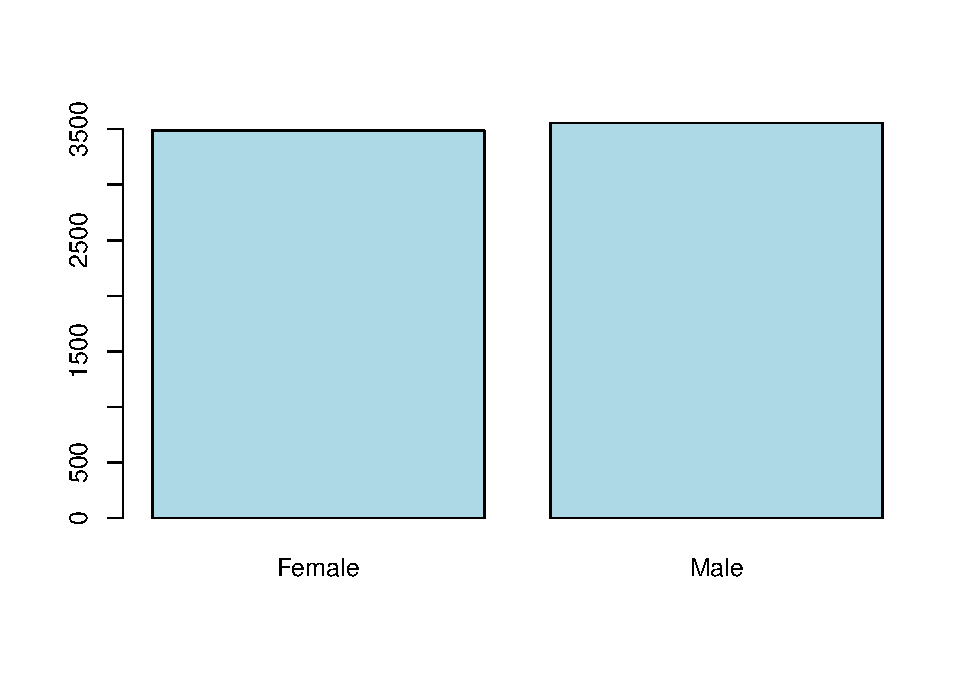
\includegraphics{Assignment2_script_files/figure-latex/unnamed-chunk-7-1.pdf}

\#Partner\\
Those are customers with partner, and we see it is pretty balanced.

\begin{Shaded}
\begin{Highlighting}[]
\NormalTok{na.partner }\OtherTok{\textless{}{-}} \FunctionTok{sum}\NormalTok{(}\FunctionTok{is.na}\NormalTok{(df}\SpecialCharTok{$}\NormalTok{Partner)) }\CommentTok{\#No NAs}
\FunctionTok{barplot}\NormalTok{(}\FunctionTok{table}\NormalTok{(df}\SpecialCharTok{$}\NormalTok{Partner),}\AttributeTok{col=}\StringTok{\textquotesingle{}lightblue\textquotesingle{}}\NormalTok{) }\CommentTok{\#Balanced}
\end{Highlighting}
\end{Shaded}

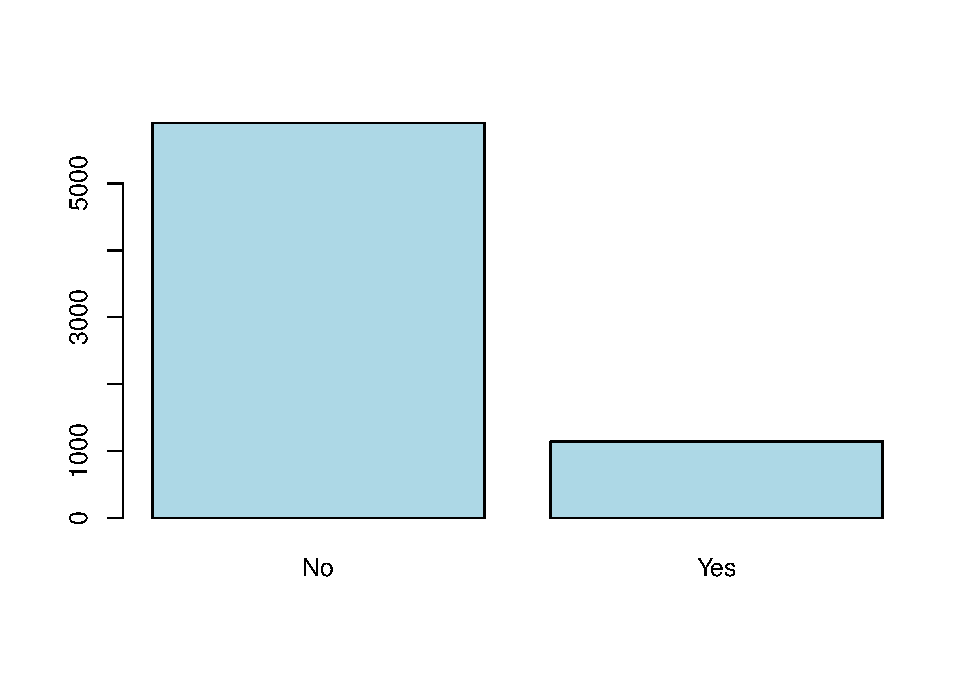
\includegraphics{Assignment2_script_files/figure-latex/unnamed-chunk-8-1.pdf}

\#Dependents\\
The dependent customers follow a similar distribution than the
SeniorCitizen.

\begin{Shaded}
\begin{Highlighting}[]
\NormalTok{na.dependents }\OtherTok{\textless{}{-}} \FunctionTok{sum}\NormalTok{(}\FunctionTok{is.na}\NormalTok{(df}\SpecialCharTok{$}\NormalTok{Dependents)) }\CommentTok{\#No NAs}
\FunctionTok{barplot}\NormalTok{(}\FunctionTok{table}\NormalTok{(df}\SpecialCharTok{$}\NormalTok{Dependents),}\AttributeTok{col=}\StringTok{\textquotesingle{}lightblue\textquotesingle{}}\NormalTok{) }\CommentTok{\#Unbalanced}
\end{Highlighting}
\end{Shaded}

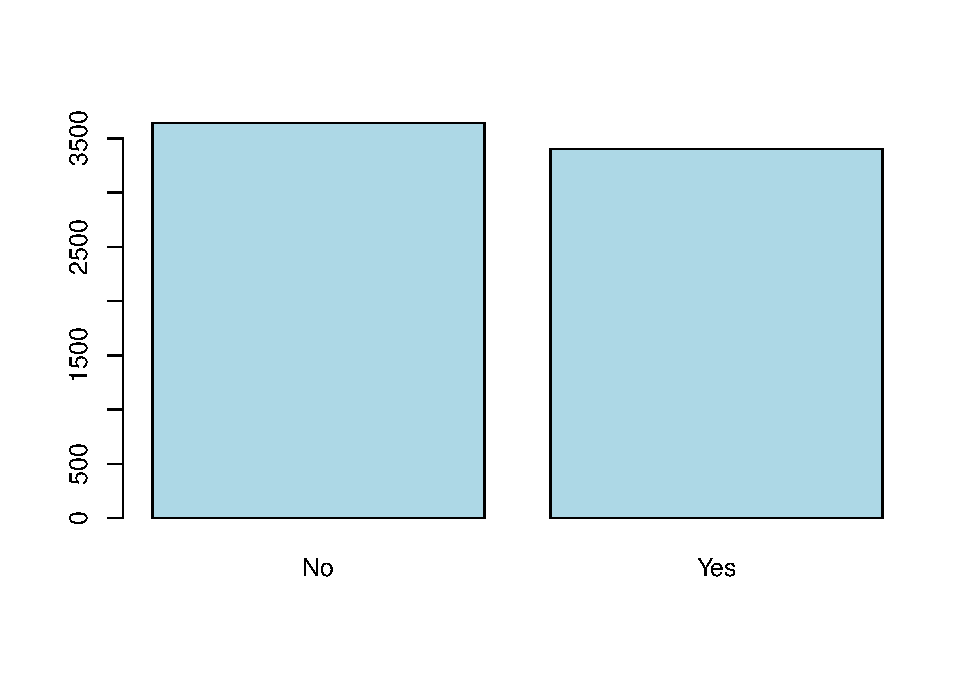
\includegraphics{Assignment2_script_files/figure-latex/unnamed-chunk-9-1.pdf}

\#Tenure\\
This is the months that a customers have been in the company. We can see
that the majority of the customer base are recent customers. We can see
that, using an Anderson-Darling test the variable is not normally
distributied, and has no univariate outliers.

\begin{Shaded}
\begin{Highlighting}[]
\NormalTok{na.tenure }\OtherTok{\textless{}{-}} \FunctionTok{sum}\NormalTok{(}\FunctionTok{is.na}\NormalTok{(df}\SpecialCharTok{$}\NormalTok{tenure)) }\CommentTok{\#No NAs}
\FunctionTok{hist}\NormalTok{(df}\SpecialCharTok{$}\NormalTok{tenure,}\AttributeTok{freq=}\NormalTok{F,}\DecValTok{15}\NormalTok{) }\CommentTok{\#Young customers overrepresented}
\NormalTok{mm }\OtherTok{\textless{}{-}} \FunctionTok{mean}\NormalTok{(df}\SpecialCharTok{$}\NormalTok{tenure,}\AttributeTok{na.rm=}\NormalTok{T);ss }\OtherTok{\textless{}{-}} \FunctionTok{sd}\NormalTok{(df}\SpecialCharTok{$}\NormalTok{tenure,}\AttributeTok{na.rm=}\NormalTok{T);}
\FunctionTok{curve}\NormalTok{(}\FunctionTok{dnorm}\NormalTok{(x,mm,ss),}\AttributeTok{col=}\StringTok{"red"}\NormalTok{,}\AttributeTok{add=}\NormalTok{T)}
\end{Highlighting}
\end{Shaded}

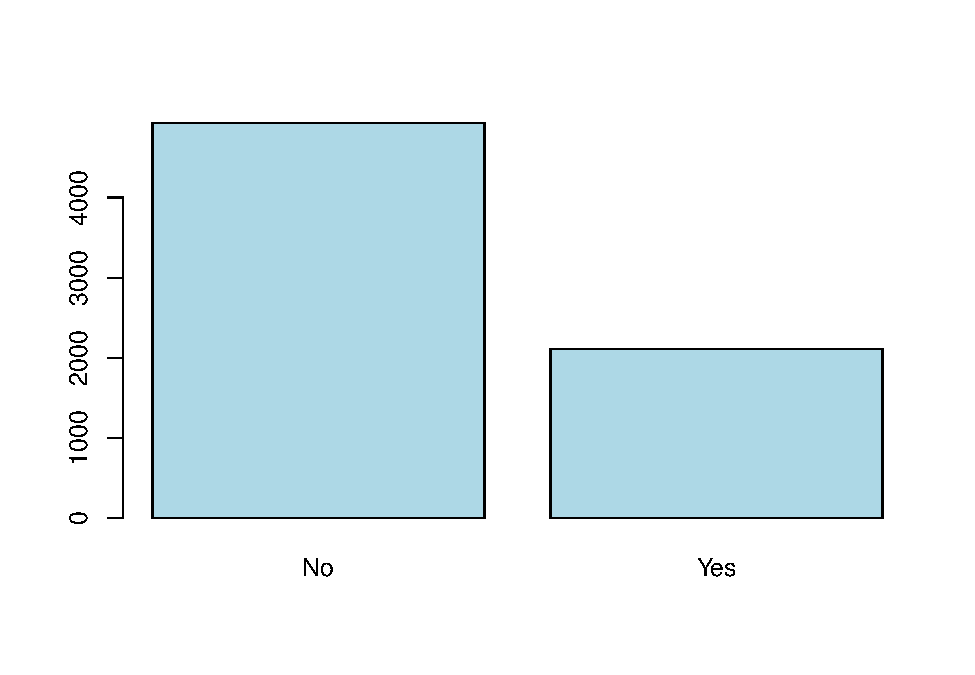
\includegraphics{Assignment2_script_files/figure-latex/unnamed-chunk-10-1.pdf}

\begin{Shaded}
\begin{Highlighting}[]
\CommentTok{\#shapiro.test(df$tenure) \#Error: too many samples for shapiro test}
\FunctionTok{ad.test}\NormalTok{(df}\SpecialCharTok{$}\NormalTok{tenure) }\CommentTok{\#Anderson{-}Darling test: Not normally distributed}
\end{Highlighting}
\end{Shaded}

\begin{verbatim}
## 
##  Anderson-Darling normality test
## 
## data:  df$tenure
## A = 203.24, p-value < 2.2e-16
\end{verbatim}

\begin{Shaded}
\begin{Highlighting}[]
\FunctionTok{Boxplot}\NormalTok{(df}\SpecialCharTok{$}\NormalTok{tenure,}\AttributeTok{range=}\FloatTok{1.5}\NormalTok{,}\AttributeTok{id=}\FunctionTok{list}\NormalTok{(}\AttributeTok{n=}\ConstantTok{Inf}\NormalTok{,}\AttributeTok{labels=}\FunctionTok{rownames}\NormalTok{(df))) }\CommentTok{\#No mild univariate outliers}
\FunctionTok{Boxplot}\NormalTok{(df}\SpecialCharTok{$}\NormalTok{tenure,}\AttributeTok{range=}\DecValTok{3}\NormalTok{,}\AttributeTok{id=}\FunctionTok{list}\NormalTok{(}\AttributeTok{n=}\ConstantTok{Inf}\NormalTok{,}\AttributeTok{labels=}\FunctionTok{rownames}\NormalTok{(df))) }\CommentTok{\#No extreme univariate outliers}
\end{Highlighting}
\end{Shaded}

\includegraphics{Assignment2_script_files/figure-latex/unnamed-chunk-10-2.pdf}

\#PhoneService\\
Now we can see that the majority of the clients have PhoneService in the
contract.

\begin{Shaded}
\begin{Highlighting}[]
\NormalTok{na.phoneservice }\OtherTok{\textless{}{-}} \FunctionTok{sum}\NormalTok{(}\FunctionTok{is.na}\NormalTok{(df}\SpecialCharTok{$}\NormalTok{PhoneService)) }\CommentTok{\#No NAs}
\FunctionTok{barplot}\NormalTok{(}\FunctionTok{table}\NormalTok{(df}\SpecialCharTok{$}\NormalTok{PhoneService),}\AttributeTok{col=}\StringTok{\textquotesingle{}lightblue\textquotesingle{}}\NormalTok{) }\CommentTok{\#Unbalanced}
\end{Highlighting}
\end{Shaded}

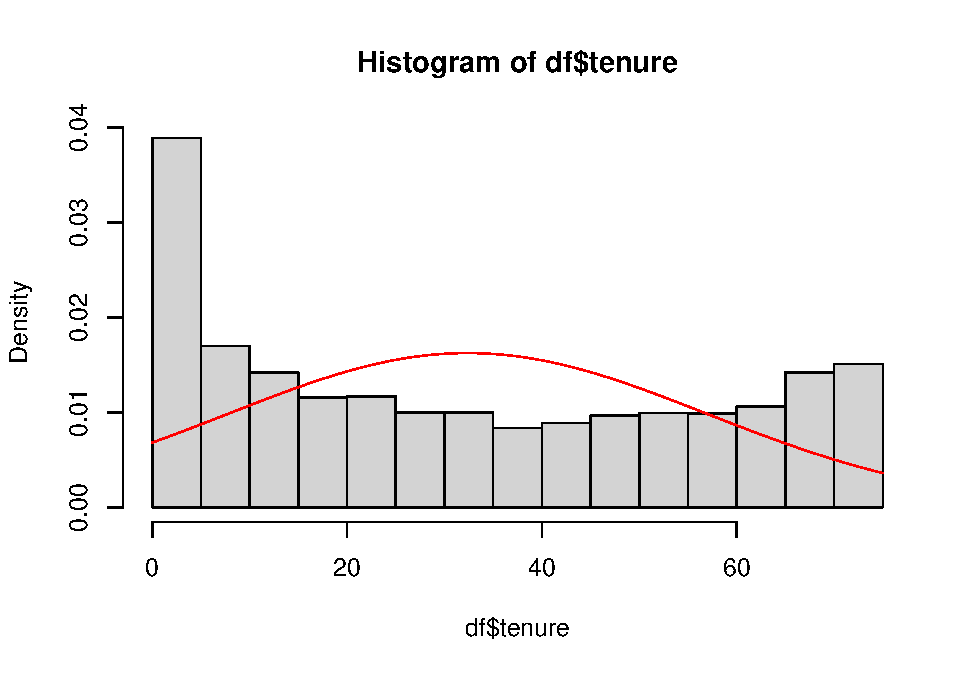
\includegraphics{Assignment2_script_files/figure-latex/unnamed-chunk-11-1.pdf}

\#MultipleLines\\
As we saw before, the majority of the clients have PhoneService, so they
are underrepresented in this variable, but regarding those who have,
MultipleLines is pretty balanced.

\begin{Shaded}
\begin{Highlighting}[]
\NormalTok{na.multiplelines }\OtherTok{\textless{}{-}} \FunctionTok{sum}\NormalTok{(}\FunctionTok{is.na}\NormalTok{(df}\SpecialCharTok{$}\NormalTok{MultipleLines)) }\CommentTok{\#No NAs}
\FunctionTok{barplot}\NormalTok{(}\FunctionTok{table}\NormalTok{(df}\SpecialCharTok{$}\NormalTok{MultipleLines),}\AttributeTok{col=}\StringTok{\textquotesingle{}lightblue\textquotesingle{}}\NormalTok{) }\CommentTok{\#Unbalanced in "No phone service"}
\end{Highlighting}
\end{Shaded}

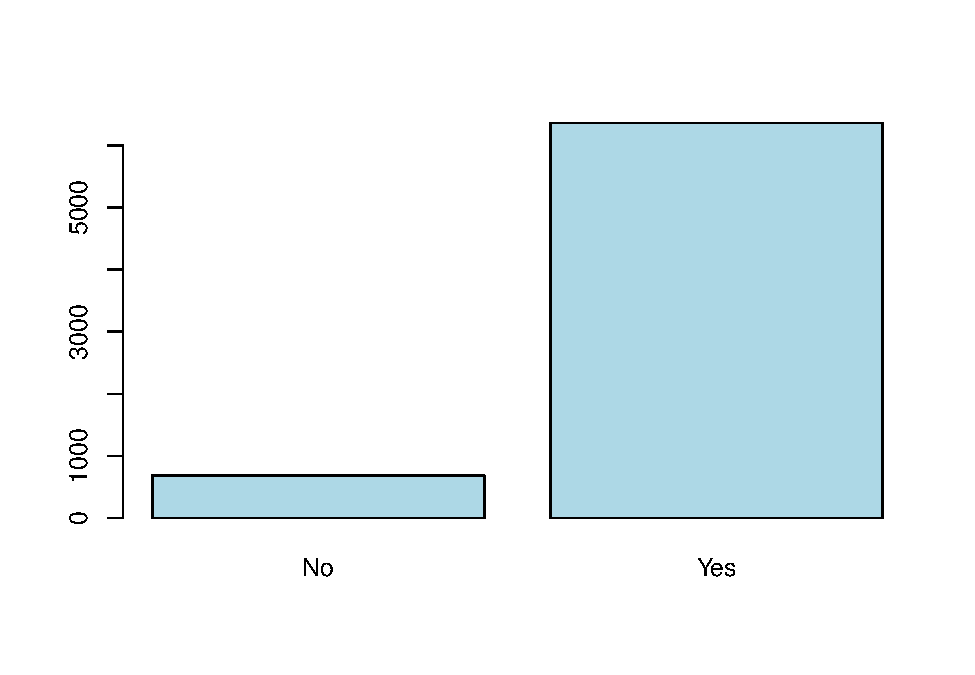
\includegraphics{Assignment2_script_files/figure-latex/unnamed-chunk-12-1.pdf}

\#InternetService\\
Most of the clients have fiber optic, and there are a few that don't
have internet service.

\begin{Shaded}
\begin{Highlighting}[]
\NormalTok{na.internetservice }\OtherTok{\textless{}{-}} \FunctionTok{sum}\NormalTok{(}\FunctionTok{is.na}\NormalTok{(df}\SpecialCharTok{$}\NormalTok{InternetService)) }\CommentTok{\#No NAs}
\FunctionTok{barplot}\NormalTok{(}\FunctionTok{table}\NormalTok{(df}\SpecialCharTok{$}\NormalTok{InternetService),}\AttributeTok{col=}\StringTok{\textquotesingle{}lightblue\textquotesingle{}}\NormalTok{) }\CommentTok{\#Unbalanced}
\end{Highlighting}
\end{Shaded}

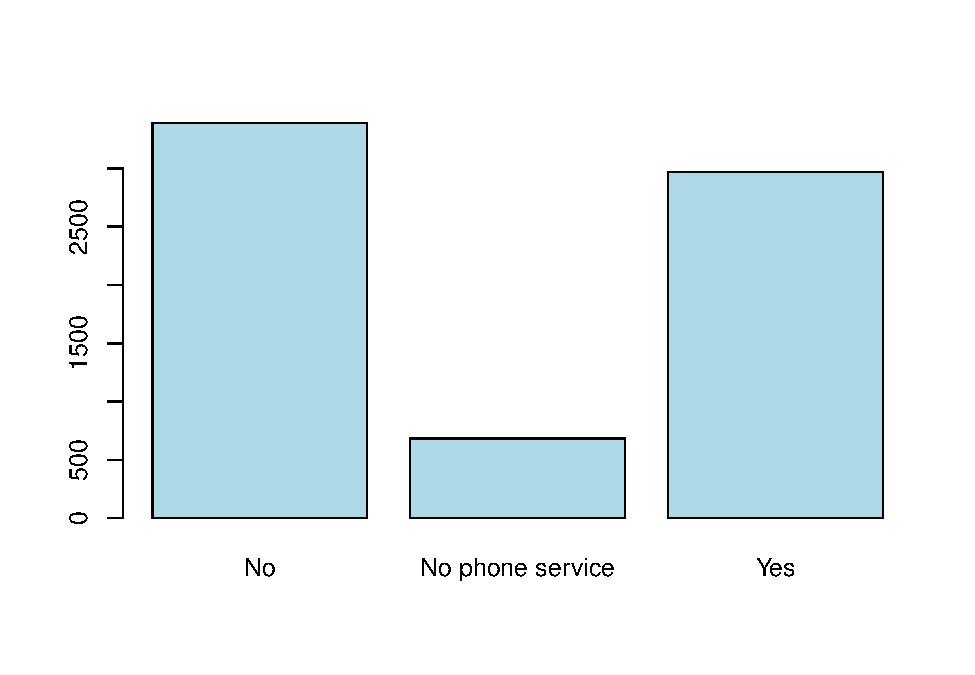
\includegraphics{Assignment2_script_files/figure-latex/unnamed-chunk-13-1.pdf}

\#OnlineSecurity\\
Those clients without internet service are a minority as they were in
the previous variable, and most of those with internet service don't
have OnlineSecurity.

\begin{Shaded}
\begin{Highlighting}[]
\NormalTok{no.onlinesecurity }\OtherTok{\textless{}{-}} \FunctionTok{sum}\NormalTok{(}\FunctionTok{is.na}\NormalTok{(df}\SpecialCharTok{$}\NormalTok{OnlineSecurity)) }\CommentTok{\#No NAs}
\FunctionTok{barplot}\NormalTok{(}\FunctionTok{table}\NormalTok{(df}\SpecialCharTok{$}\NormalTok{OnlineSecurity),}\AttributeTok{col=}\StringTok{\textquotesingle{}lightblue\textquotesingle{}}\NormalTok{) }\CommentTok{\#Unbalanced in "No"}
\end{Highlighting}
\end{Shaded}

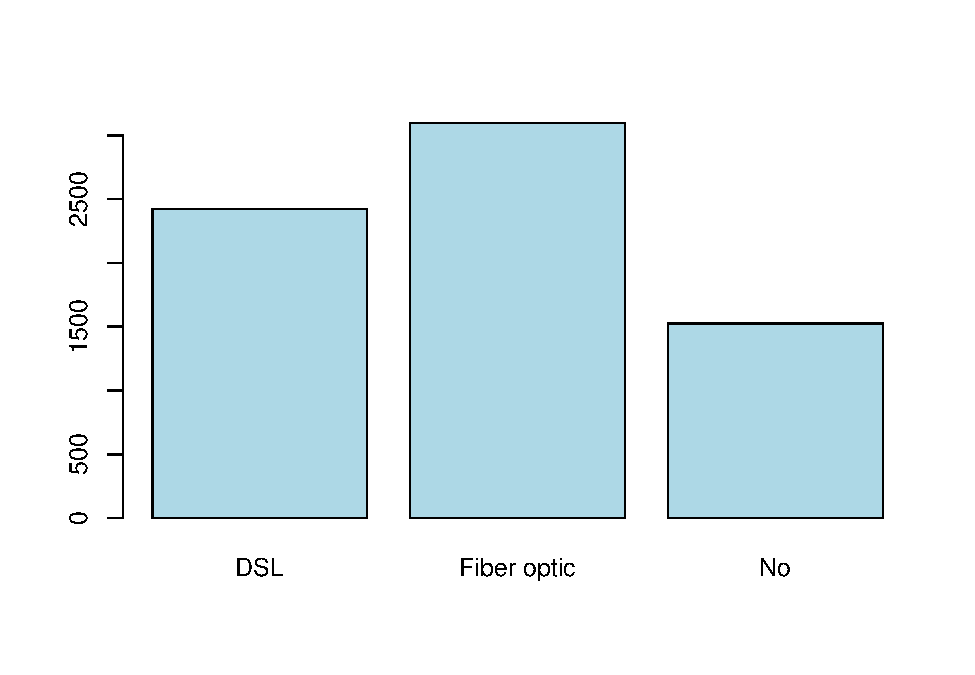
\includegraphics{Assignment2_script_files/figure-latex/unnamed-chunk-14-1.pdf}

\#OnlineBackup\\
Similar to previous variable

\begin{Shaded}
\begin{Highlighting}[]
\NormalTok{na.onlinebackup }\OtherTok{\textless{}{-}} \FunctionTok{sum}\NormalTok{(}\FunctionTok{is.na}\NormalTok{(df}\SpecialCharTok{$}\NormalTok{OnlineBackup)) }\CommentTok{\#No NAs}
\FunctionTok{barplot}\NormalTok{(}\FunctionTok{table}\NormalTok{(df}\SpecialCharTok{$}\NormalTok{OnlineBackup),}\AttributeTok{col=}\StringTok{\textquotesingle{}lightblue\textquotesingle{}}\NormalTok{) }\CommentTok{\#Unbalanced}
\end{Highlighting}
\end{Shaded}

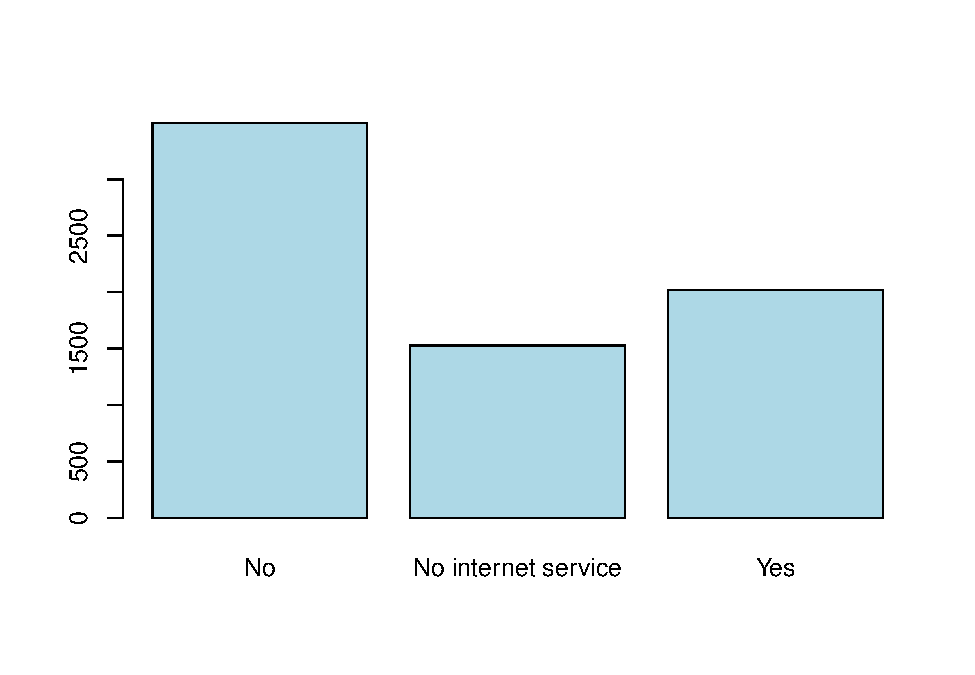
\includegraphics{Assignment2_script_files/figure-latex/unnamed-chunk-15-1.pdf}

\#DeviceProtection\\
Similar to previous variable

\begin{Shaded}
\begin{Highlighting}[]
\NormalTok{na.deviceprotection }\OtherTok{\textless{}{-}} \FunctionTok{sum}\NormalTok{(}\FunctionTok{is.na}\NormalTok{(df}\SpecialCharTok{$}\NormalTok{DeviceProtection)) }\CommentTok{\#No NAs}
\FunctionTok{barplot}\NormalTok{(}\FunctionTok{table}\NormalTok{(df}\SpecialCharTok{$}\NormalTok{DeviceProtection),}\AttributeTok{col=}\StringTok{\textquotesingle{}lightblue\textquotesingle{}}\NormalTok{) }\CommentTok{\#Unbalanced}
\end{Highlighting}
\end{Shaded}

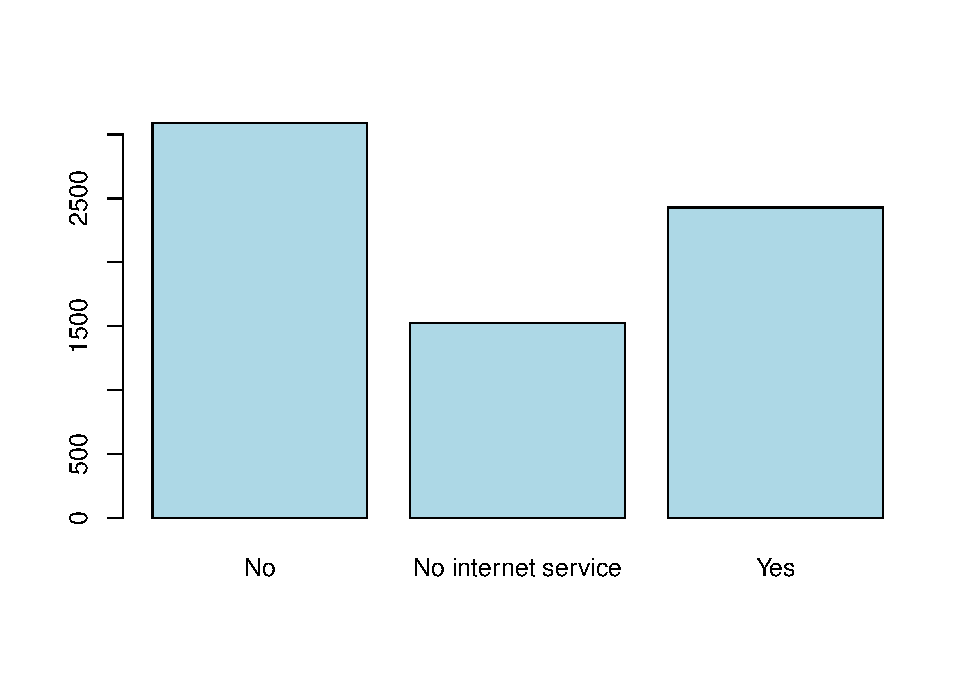
\includegraphics{Assignment2_script_files/figure-latex/unnamed-chunk-16-1.pdf}

\#TechSupport\\
Similar to previous variable

\begin{Shaded}
\begin{Highlighting}[]
\NormalTok{na.techsupport }\OtherTok{\textless{}{-}} \FunctionTok{sum}\NormalTok{(}\FunctionTok{is.na}\NormalTok{(df}\SpecialCharTok{$}\NormalTok{TechSupport)) }\CommentTok{\#No NAs}
\FunctionTok{barplot}\NormalTok{(}\FunctionTok{table}\NormalTok{(df}\SpecialCharTok{$}\NormalTok{TechSupport),}\AttributeTok{col=}\StringTok{\textquotesingle{}lightblue\textquotesingle{}}\NormalTok{) }\CommentTok{\#Unbalanced in "No"}
\end{Highlighting}
\end{Shaded}

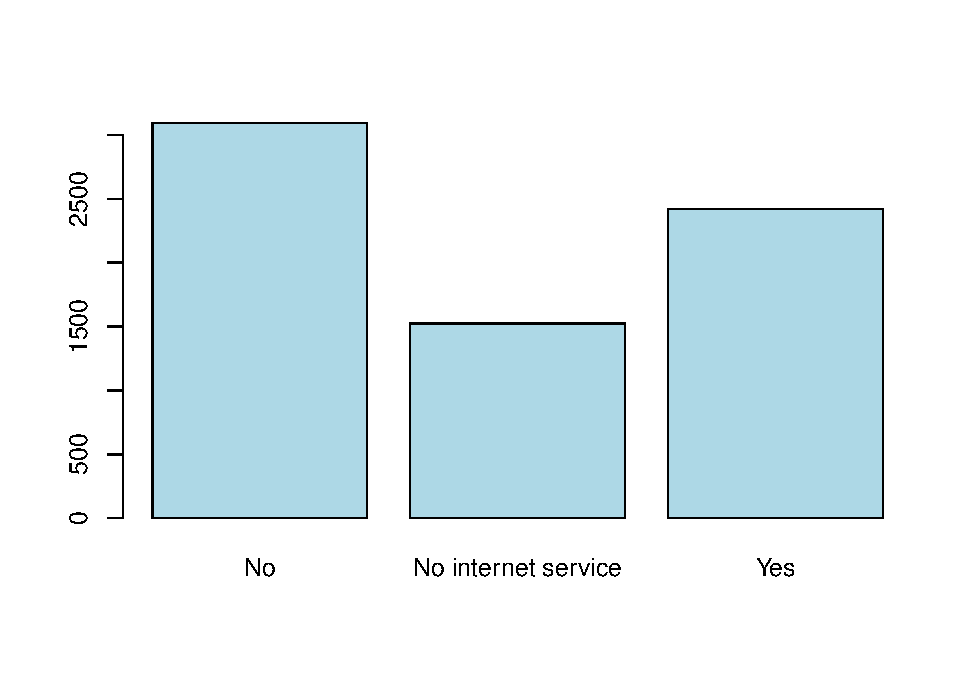
\includegraphics{Assignment2_script_files/figure-latex/unnamed-chunk-17-1.pdf}

\#StreamingMovies\\
In this case, disregarding the users without internet service, the
categories are balanced.

\begin{Shaded}
\begin{Highlighting}[]
\NormalTok{na.streamingmovies }\OtherTok{\textless{}{-}} \FunctionTok{sum}\NormalTok{(}\FunctionTok{is.na}\NormalTok{(df}\SpecialCharTok{$}\NormalTok{StreamingMovies)) }\CommentTok{\#No NAs}
\FunctionTok{barplot}\NormalTok{(}\FunctionTok{table}\NormalTok{(df}\SpecialCharTok{$}\NormalTok{StreamingMovies),}\AttributeTok{col=}\StringTok{\textquotesingle{}lightblue\textquotesingle{}}\NormalTok{) }\CommentTok{\#Unbalanced in "No internet service"}
\end{Highlighting}
\end{Shaded}

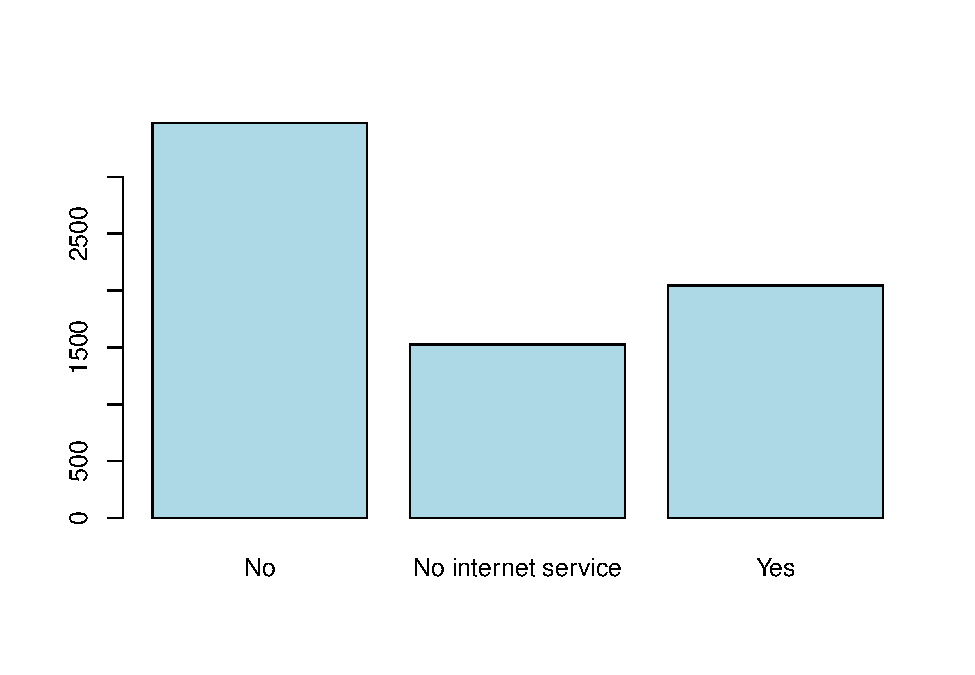
\includegraphics{Assignment2_script_files/figure-latex/unnamed-chunk-18-1.pdf}

\#Contract\\
Most of the contracts are month to month.

\begin{Shaded}
\begin{Highlighting}[]
\NormalTok{na.contract }\OtherTok{\textless{}{-}} \FunctionTok{sum}\NormalTok{(}\FunctionTok{is.na}\NormalTok{(df}\SpecialCharTok{$}\NormalTok{Contract)) }\CommentTok{\#No NAs}
\FunctionTok{barplot}\NormalTok{(}\FunctionTok{table}\NormalTok{(df}\SpecialCharTok{$}\NormalTok{Contract),}\AttributeTok{col=}\StringTok{\textquotesingle{}lightblue\textquotesingle{}}\NormalTok{) }\CommentTok{\#Unbalanced in "Month{-}to{-}month"}
\end{Highlighting}
\end{Shaded}

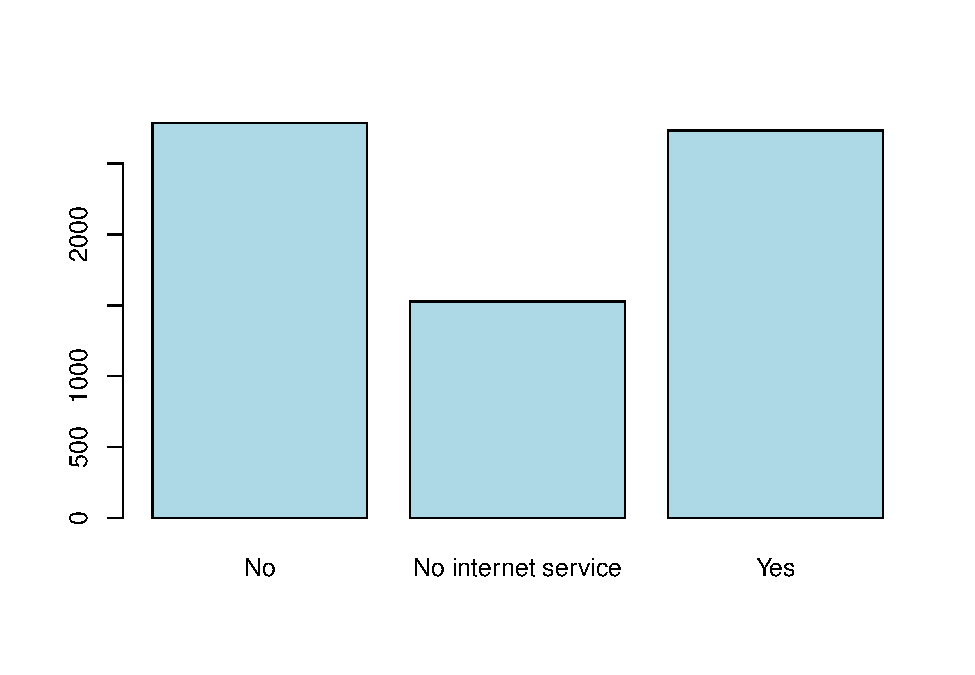
\includegraphics{Assignment2_script_files/figure-latex/unnamed-chunk-19-1.pdf}

\#PaperlessBilling\\
This variable is pretty much balanced, with more population towards
having PaperlessBilling.

\begin{Shaded}
\begin{Highlighting}[]
\NormalTok{na.paperlessbilling }\OtherTok{\textless{}{-}} \FunctionTok{sum}\NormalTok{(}\FunctionTok{is.na}\NormalTok{(df}\SpecialCharTok{$}\NormalTok{PaperlessBilling)) }\CommentTok{\#No NAs}
\FunctionTok{barplot}\NormalTok{(}\FunctionTok{table}\NormalTok{(df}\SpecialCharTok{$}\NormalTok{PaperlessBilling),}\AttributeTok{col=}\StringTok{\textquotesingle{}lightblue\textquotesingle{}}\NormalTok{) }\CommentTok{\#Relatively balanced}
\end{Highlighting}
\end{Shaded}

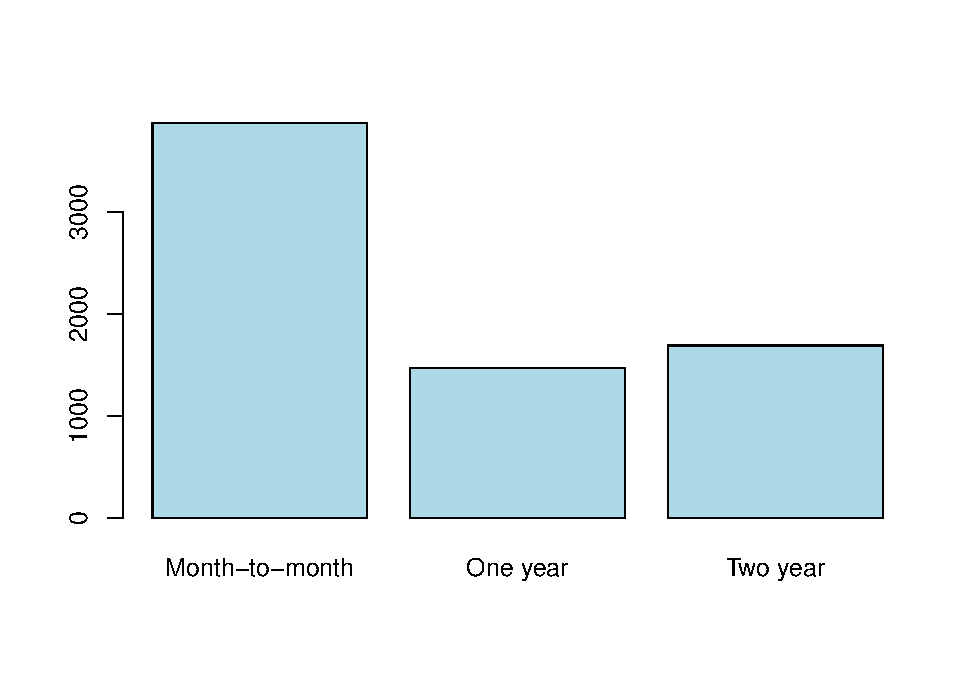
\includegraphics{Assignment2_script_files/figure-latex/unnamed-chunk-20-1.pdf}

\#PaymentMethod\\
Most of the customers use electronic check.

\begin{Shaded}
\begin{Highlighting}[]
\NormalTok{na.paymentmethod }\OtherTok{\textless{}{-}} \FunctionTok{sum}\NormalTok{(}\FunctionTok{is.na}\NormalTok{(df}\SpecialCharTok{$}\NormalTok{PaymentMethod)) }\CommentTok{\#No NAs}
\FunctionTok{barplot}\NormalTok{(}\FunctionTok{table}\NormalTok{(df}\SpecialCharTok{$}\NormalTok{PaymentMethod),}\AttributeTok{col=}\StringTok{\textquotesingle{}lightblue\textquotesingle{}}\NormalTok{) }\CommentTok{\#Unbalanced in "Electronic check"}
\end{Highlighting}
\end{Shaded}

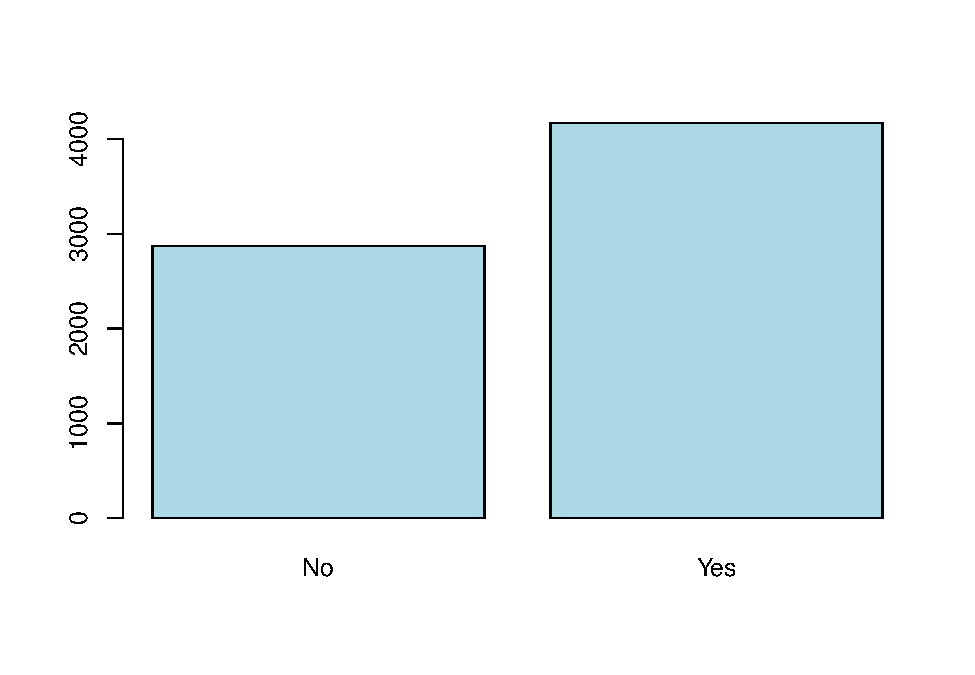
\includegraphics{Assignment2_script_files/figure-latex/unnamed-chunk-21-1.pdf}

\#MonthlyCharges\\
We can see that most of population concentrates around 20 units of
MothlyCharges. Not normally distributed. No univariate outliers.

\begin{Shaded}
\begin{Highlighting}[]
\NormalTok{na.monthlycharges }\OtherTok{\textless{}{-}} \FunctionTok{sum}\NormalTok{(}\FunctionTok{is.na}\NormalTok{(df}\SpecialCharTok{$}\NormalTok{MonthlyCharges)) }\CommentTok{\#No NAs}
\FunctionTok{hist}\NormalTok{(df}\SpecialCharTok{$}\NormalTok{MonthlyCharges,}\AttributeTok{freq=}\NormalTok{F,}\DecValTok{15}\NormalTok{)}
\NormalTok{mm }\OtherTok{\textless{}{-}} \FunctionTok{mean}\NormalTok{(df}\SpecialCharTok{$}\NormalTok{MonthlyCharges,}\AttributeTok{na.rm=}\NormalTok{T)}
\NormalTok{ss }\OtherTok{\textless{}{-}} \FunctionTok{sd}\NormalTok{(df}\SpecialCharTok{$}\NormalTok{MonthlyCharges,}\AttributeTok{na.rm=}\NormalTok{T)}
\FunctionTok{curve}\NormalTok{(}\FunctionTok{dnorm}\NormalTok{(x,mm,ss),}\AttributeTok{col=}\StringTok{"red"}\NormalTok{,}\AttributeTok{add=}\NormalTok{T)}
\end{Highlighting}
\end{Shaded}

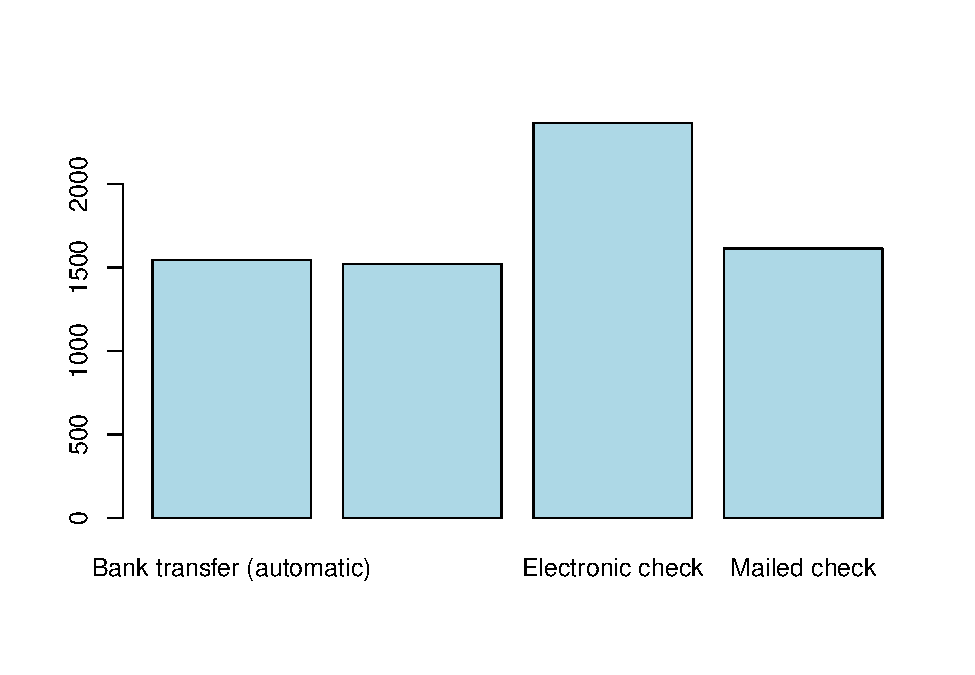
\includegraphics{Assignment2_script_files/figure-latex/unnamed-chunk-22-1.pdf}

\begin{Shaded}
\begin{Highlighting}[]
\CommentTok{\#shapiro.test(df$MonthlyCharges) \#Error: too many samples for shapiro test}
\FunctionTok{ad.test}\NormalTok{(df}\SpecialCharTok{$}\NormalTok{MonthlyCharges) }\CommentTok{\#Anderson{-}Darling test: Not normally distributed}
\end{Highlighting}
\end{Shaded}

\begin{verbatim}
## 
##  Anderson-Darling normality test
## 
## data:  df$MonthlyCharges
## A = 170.56, p-value < 2.2e-16
\end{verbatim}

\begin{Shaded}
\begin{Highlighting}[]
\FunctionTok{Boxplot}\NormalTok{(df}\SpecialCharTok{$}\NormalTok{MonthlyCharges,}\AttributeTok{range=}\FloatTok{1.5}\NormalTok{,}\AttributeTok{id=}\FunctionTok{list}\NormalTok{(}\AttributeTok{n=}\ConstantTok{Inf}\NormalTok{,}\AttributeTok{labels=}\FunctionTok{rownames}\NormalTok{(df))) }\CommentTok{\#No mild univariate outliers}
\FunctionTok{Boxplot}\NormalTok{(df}\SpecialCharTok{$}\NormalTok{MonthlyCharges,}\AttributeTok{range=}\DecValTok{3}\NormalTok{,}\AttributeTok{id=}\FunctionTok{list}\NormalTok{(}\AttributeTok{n=}\ConstantTok{Inf}\NormalTok{,}\AttributeTok{labels=}\FunctionTok{rownames}\NormalTok{(df))) }\CommentTok{\#No severe univariate outliers}
\end{Highlighting}
\end{Shaded}

\includegraphics{Assignment2_script_files/figure-latex/unnamed-chunk-22-2.pdf}

\#TotalCharges\\
Again, most of the population groups around small values. Not normally
distributed. No univariate outliers.

\begin{Shaded}
\begin{Highlighting}[]
\NormalTok{na.totalcharges }\OtherTok{\textless{}{-}} \FunctionTok{sum}\NormalTok{(}\FunctionTok{is.na}\NormalTok{(df}\SpecialCharTok{$}\NormalTok{TotalCharges)) }\CommentTok{\#11 NAs imputed earlier}
\FunctionTok{hist}\NormalTok{(df}\SpecialCharTok{$}\NormalTok{TotalCharges,}\AttributeTok{freq=}\NormalTok{F,}\DecValTok{15}\NormalTok{)}
\NormalTok{mm }\OtherTok{\textless{}{-}} \FunctionTok{mean}\NormalTok{(df}\SpecialCharTok{$}\NormalTok{TotalCharges,}\AttributeTok{na.rm=}\NormalTok{T)}
\NormalTok{ss }\OtherTok{\textless{}{-}} \FunctionTok{sd}\NormalTok{(df}\SpecialCharTok{$}\NormalTok{TotalCharges,}\AttributeTok{na.rm=}\NormalTok{T)}
\FunctionTok{curve}\NormalTok{(}\FunctionTok{dnorm}\NormalTok{(x,mm,ss),}\AttributeTok{col=}\StringTok{"red"}\NormalTok{,}\AttributeTok{add=}\NormalTok{T)}
\end{Highlighting}
\end{Shaded}

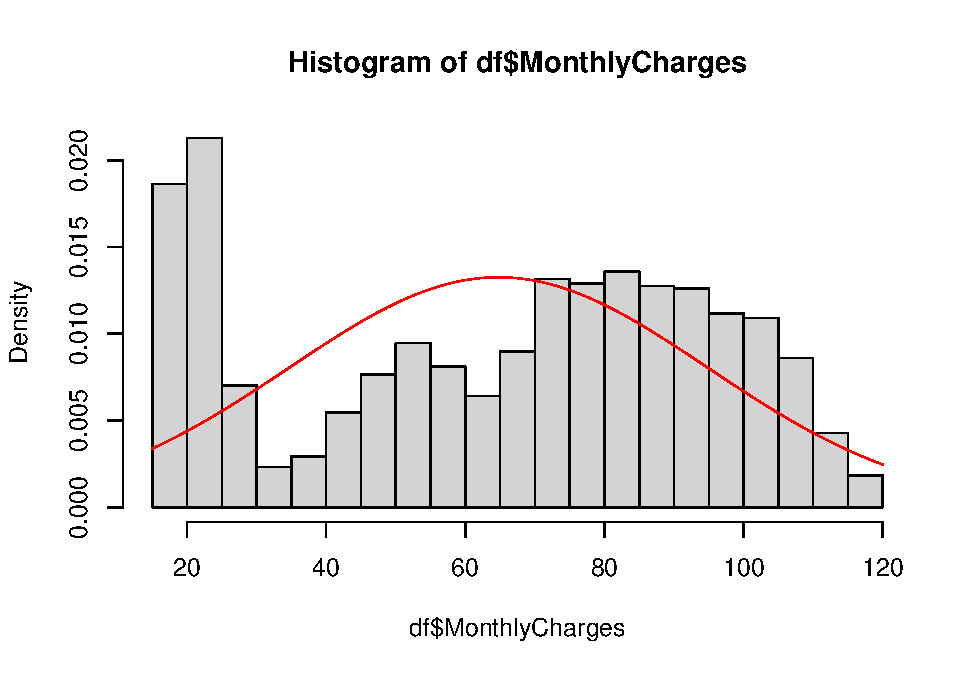
\includegraphics{Assignment2_script_files/figure-latex/unnamed-chunk-23-1.pdf}

\begin{Shaded}
\begin{Highlighting}[]
\CommentTok{\#shapiro.test(df$TotalCharges) \#Error: too many samples for shapiro test}
\FunctionTok{ad.test}\NormalTok{(df}\SpecialCharTok{$}\NormalTok{TotalCharges) }\CommentTok{\#Anderson{-}Darling test: Not normally distributed}
\end{Highlighting}
\end{Shaded}

\begin{verbatim}
## 
##  Anderson-Darling normality test
## 
## data:  df$TotalCharges
## A = 346.64, p-value < 2.2e-16
\end{verbatim}

\begin{Shaded}
\begin{Highlighting}[]
\FunctionTok{Boxplot}\NormalTok{(df}\SpecialCharTok{$}\NormalTok{TotalCharges,}\AttributeTok{range=}\FloatTok{1.5}\NormalTok{,}\AttributeTok{id=}\FunctionTok{list}\NormalTok{(}\AttributeTok{n=}\ConstantTok{Inf}\NormalTok{,}\AttributeTok{labels=}\FunctionTok{rownames}\NormalTok{(df))) }\CommentTok{\#No mild univariate outliers}
\FunctionTok{Boxplot}\NormalTok{(df}\SpecialCharTok{$}\NormalTok{TotalCharges,}\AttributeTok{range=}\DecValTok{3}\NormalTok{,}\AttributeTok{id=}\FunctionTok{list}\NormalTok{(}\AttributeTok{n=}\ConstantTok{Inf}\NormalTok{,}\AttributeTok{labels=}\FunctionTok{rownames}\NormalTok{(df))) }\CommentTok{\#No severe univariate outliers}
\end{Highlighting}
\end{Shaded}

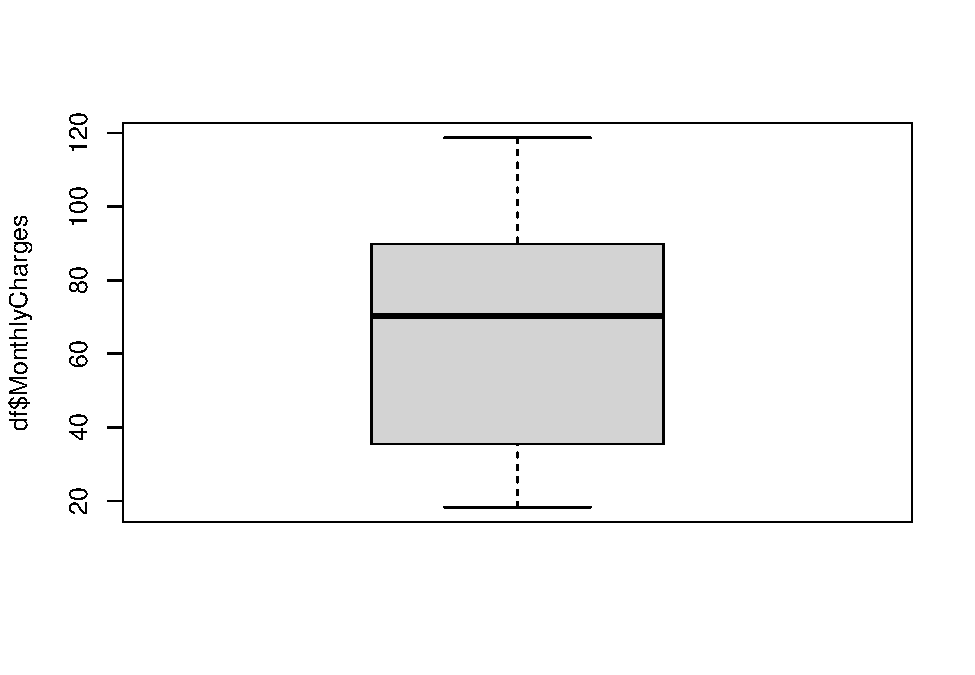
\includegraphics{Assignment2_script_files/figure-latex/unnamed-chunk-23-2.pdf}

\hypertarget{profiling-target-variable-churn}{%
\section{Profiling Target Variable:
Churn}\label{profiling-target-variable-churn}}

We can see from the summary of the target variable Churn that it is
highly unbalanced. 73\% of all instances do not Churn. This may be a
problem when building a model that we must keep in mind.

Using catdes we can see that the most highly related categorical
variables are Contract, OnlineSecurity, TechSupport, InternetService,
PaymentMethod, ONlineBackup, DeviceProtection, StreamingMovies,
StreamingTV, PaperlessBilling, Dependents, SeniorCitizen, Partner, and
MultipleLines. All of these variables also have an extremely low p-value
(far below the 5\% significance level) which indicates a strong link to
the target. For the quantitative variables, we can see that the target
Churn is highly linked to all the numeric variables, tenure,
TotalCharges, and MonthlyCharges.

\begin{Shaded}
\begin{Highlighting}[]
\NormalTok{na.churn }\OtherTok{\textless{}{-}} \FunctionTok{sum}\NormalTok{(}\FunctionTok{is.na}\NormalTok{(df}\SpecialCharTok{$}\NormalTok{Churn)) }\CommentTok{\#No NAs}
\FunctionTok{summary}\NormalTok{(df}\SpecialCharTok{$}\NormalTok{Churn)}
\end{Highlighting}
\end{Shaded}

\begin{verbatim}
##   No  Yes 
## 5174 1869
\end{verbatim}

\begin{Shaded}
\begin{Highlighting}[]
\NormalTok{ptt}\OtherTok{\textless{}{-}}\FunctionTok{prop.table}\NormalTok{(}\FunctionTok{table}\NormalTok{(df}\SpecialCharTok{$}\NormalTok{Churn));ptt}
\end{Highlighting}
\end{Shaded}

\begin{verbatim}
## 
##        No       Yes 
## 0.7346301 0.2653699
\end{verbatim}

\begin{Shaded}
\begin{Highlighting}[]
\FunctionTok{barplot}\NormalTok{(}\FunctionTok{table}\NormalTok{(df}\SpecialCharTok{$}\NormalTok{Churn),}\AttributeTok{col=}\StringTok{\textquotesingle{}lightblue\textquotesingle{}}\NormalTok{) }\CommentTok{\#Unbalanced}
\end{Highlighting}
\end{Shaded}

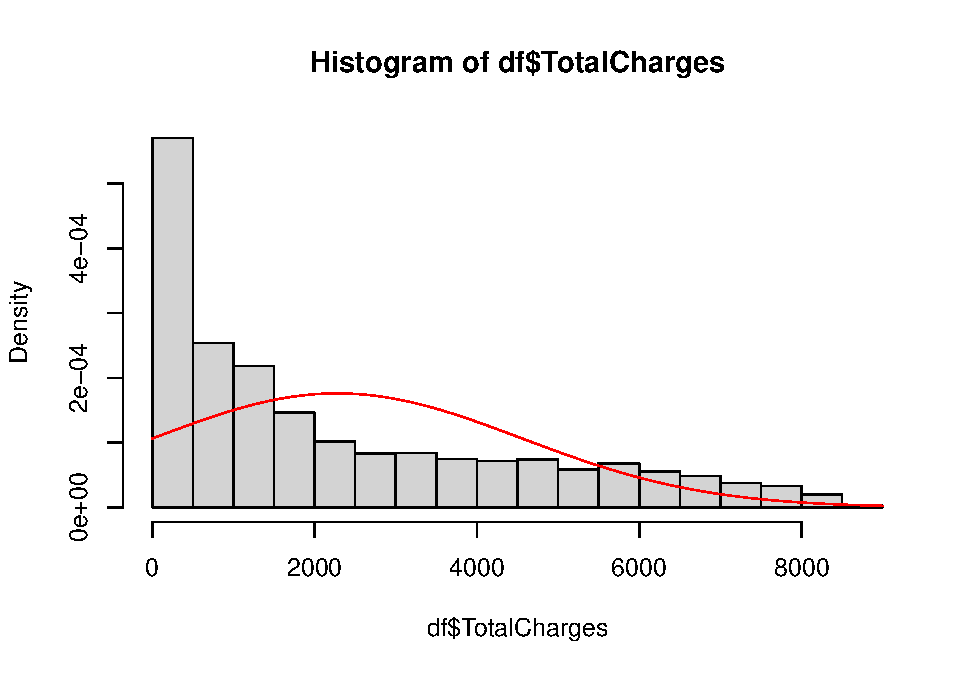
\includegraphics{Assignment2_script_files/figure-latex/unnamed-chunk-24-1.pdf}

\begin{Shaded}
\begin{Highlighting}[]
\FunctionTok{catdes}\NormalTok{(df,}\DecValTok{21}\NormalTok{)}
\end{Highlighting}
\end{Shaded}

\begin{verbatim}
## 
## Link between the cluster variable and the categorical variables (chi-square test)
## =================================================================================
##                        p.value df
## Contract         5.863038e-258  2
## OnlineSecurity   2.661150e-185  2
## TechSupport      1.443084e-180  2
## InternetService  9.571788e-160  2
## PaymentMethod    3.682355e-140  3
## OnlineBackup     2.079759e-131  2
## DeviceProtection 5.505219e-122  2
## StreamingMovies   2.667757e-82  2
## StreamingTV       5.528994e-82  2
## PaperlessBilling  2.614597e-58  1
## Dependents        3.276083e-43  1
## SeniorCitizen     9.477904e-37  1
## Partner           1.519037e-36  1
## MultipleLines     3.464383e-03  2
## 
## Description of each cluster by the categories
## =============================================
## $No
##                                          Cla/Mod  Mod/Cla   Global
## Contract=Two year                       97.16814 31.83224 24.06645
## StreamingMovies=No internet service     92.59502 27.30963 21.66690
## StreamingTV=No internet service         92.59502 27.30963 21.66690
## TechSupport=No internet service         92.59502 27.30963 21.66690
## DeviceProtection=No internet service    92.59502 27.30963 21.66690
## OnlineBackup=No internet service        92.59502 27.30963 21.66690
## OnlineSecurity=No internet service      92.59502 27.30963 21.66690
## InternetService=No                      92.59502 27.30963 21.66690
## PaperlessBilling=No                     83.66992 46.44376 40.77808
## Contract=One year                       88.73048 25.26092 20.91438
## OnlineSecurity=Yes                      85.38881 33.32045 28.66676
## TechSupport=Yes                         84.83366 33.51372 29.02172
## Dependents=Yes                          84.54976 34.48009 29.95882
## Partner=Yes                             80.33510 52.82180 48.30328
## SeniorCitizen=No                        76.39383 87.12795 83.78532
## PaymentMethod=Credit card (automatic)   84.75690 24.93235 21.61011
## InternetService=DSL                     81.04089 37.92037 34.37456
## PaymentMethod=Bank transfer (automatic) 83.29016 24.85504 21.92248
## PaymentMethod=Mailed check              80.89330 25.20294 22.88797
## OnlineBackup=Yes                        78.46851 36.83804 34.48814
## DeviceProtection=Yes                    77.49794 36.27754 34.38875
## MultipleLines=No                        74.95575 49.11094 48.13290
## MultipleLines=Yes                       71.39010 40.99343 42.18373
## StreamingMovies=Yes                     70.05857 36.99266 38.79029
## StreamingTV=Yes                         69.92981 36.58678 38.43533
## StreamingTV=No                          66.47687 36.10359 39.89777
## StreamingMovies=No                      66.31957 35.69772 39.54281
## SeniorCitizen=Yes                       58.31874 12.87205 16.21468
## Partner=No                              67.04202 47.17820 51.69672
## Dependents=No                           68.72086 65.51991 70.04118
## PaperlessBilling=Yes                    66.43491 53.55624 59.22192
## DeviceProtection=No                     60.87237 36.41283 43.94434
## OnlineBackup=No                         60.07124 35.85234 43.84495
## PaymentMethod=Electronic check          54.71459 25.00966 33.57944
## InternetService=Fiber optic             58.10724 34.77000 43.95854
## TechSupport=No                          58.36453 39.17665 49.31137
## OnlineSecurity=No                       58.23328 39.36993 49.66634
## Contract=Month-to-month                 57.29032 42.90684 55.01917
##                                               p.value     v.test
## Contract=Two year                       3.588830e-187  29.178937
## StreamingMovies=No internet service      6.584621e-98  20.999812
## StreamingTV=No internet service          6.584621e-98  20.999812
## TechSupport=No internet service          6.584621e-98  20.999812
## DeviceProtection=No internet service     6.584621e-98  20.999812
## OnlineBackup=No internet service         6.584621e-98  20.999812
## OnlineSecurity=No internet service       6.584621e-98  20.999812
## InternetService=No                       6.584621e-98  20.999812
## PaperlessBilling=No                      1.072745e-60  16.435085
## Contract=One year                        3.593041e-57  15.935502
## OnlineSecurity=Yes                       1.606459e-50  14.947938
## TechSupport=Yes                          1.323174e-46  14.334963
## Dependents=Yes                           3.572324e-46  14.265846
## Partner=Yes                              6.170871e-37  12.696658
## SeniorCitizen=No                         3.024931e-34  12.202212
## PaymentMethod=Credit card (automatic)    6.408166e-32  11.758206
## InternetService=DSL                      2.545367e-26  10.614727
## PaymentMethod=Bank transfer (automatic)  1.180908e-24  10.250207
## PaymentMethod=Mailed check               3.226893e-15   7.881803
## OnlineBackup=Yes                         3.021982e-12   6.976698
## DeviceProtection=Yes                     2.173366e-08   5.597602
## MultipleLines=No                         6.262488e-03   2.733712
## MultipleLines=Yes                        7.843169e-04  -3.358271
## StreamingMovies=Yes                      2.922571e-07  -5.128373
## StreamingTV=Yes                          1.283457e-07  -5.281193
## StreamingTV=No                           6.049871e-27 -10.748094
## StreamingMovies=No                       1.092934e-27 -10.904833
## SeniorCitizen=Yes                        3.024931e-34 -12.202212
## Partner=No                               6.170871e-37 -12.696658
## Dependents=No                            3.572324e-46 -14.265846
## PaperlessBilling=Yes                     1.072745e-60 -16.435085
## DeviceProtection=No                      1.116896e-99 -21.192627
## OnlineBackup=No                         3.366400e-112 -22.509287
## PaymentMethod=Electronic check          1.790860e-136 -24.864755
## InternetService=Fiber optic             2.289126e-148 -25.941138
## TechSupport=No                          1.899538e-183 -28.883947
## OnlineSecurity=No                       6.171504e-190 -29.396034
## Contract=Month-to-month                 3.620915e-283 -35.959308
## 
## $Yes
##                                           Cla/Mod   Mod/Cla   Global
## Contract=Month-to-month                 42.709677 88.550027 55.01917
## OnlineSecurity=No                       41.766724 78.170144 49.66634
## TechSupport=No                          41.635474 77.367576 49.31137
## InternetService=Fiber optic             41.892765 69.395399 43.95854
## PaymentMethod=Electronic check          45.285412 57.303371 33.57944
## OnlineBackup=No                         39.928756 65.971108 43.84495
## DeviceProtection=No                     39.127625 64.794007 43.94434
## PaperlessBilling=Yes                    33.565092 74.906367 59.22192
## Dependents=No                           31.279140 82.557517 70.04118
## Partner=No                              32.957979 64.205457 51.69672
## SeniorCitizen=Yes                       41.681261 25.468165 16.21468
## StreamingMovies=No                      33.680431 50.187266 39.54281
## StreamingTV=No                          33.523132 50.401284 39.89777
## StreamingTV=Yes                         30.070188 43.552702 38.43533
## StreamingMovies=Yes                     29.941435 43.766720 38.79029
## MultipleLines=Yes                       28.609896 45.478866 42.18373
## MultipleLines=No                        25.044248 45.425361 48.13290
## DeviceProtection=Yes                    22.502064 29.159979 34.38875
## OnlineBackup=Yes                        21.531494 27.982879 34.48814
## PaymentMethod=Mailed check              19.106700 16.479401 22.88797
## PaymentMethod=Bank transfer (automatic) 16.709845 13.804173 21.92248
## InternetService=DSL                     18.959108 24.558587 34.37456
## PaymentMethod=Credit card (automatic)   15.243101 12.413055 21.61011
## SeniorCitizen=No                        23.606168 74.531835 83.78532
## Partner=Yes                             19.664903 35.794543 48.30328
## Dependents=Yes                          15.450237 17.442483 29.95882
## TechSupport=Yes                         15.166341 16.586410 29.02172
## OnlineSecurity=Yes                      14.611194 15.783842 28.66676
## Contract=One year                       11.269518  8.881755 20.91438
## PaperlessBilling=No                     16.330084 25.093633 40.77808
## StreamingMovies=No internet service      7.404980  6.046014 21.66690
## StreamingTV=No internet service          7.404980  6.046014 21.66690
## TechSupport=No internet service          7.404980  6.046014 21.66690
## DeviceProtection=No internet service     7.404980  6.046014 21.66690
## OnlineBackup=No internet service         7.404980  6.046014 21.66690
## OnlineSecurity=No internet service       7.404980  6.046014 21.66690
## InternetService=No                       7.404980  6.046014 21.66690
## Contract=Two year                        2.831858  2.568218 24.06645
##                                               p.value     v.test
## Contract=Month-to-month                 3.620915e-283  35.959308
## OnlineSecurity=No                       6.171504e-190  29.396034
## TechSupport=No                          1.899538e-183  28.883947
## InternetService=Fiber optic             2.289126e-148  25.941138
## PaymentMethod=Electronic check          1.790860e-136  24.864755
## OnlineBackup=No                         3.366400e-112  22.509287
## DeviceProtection=No                      1.116896e-99  21.192627
## PaperlessBilling=Yes                     1.072745e-60  16.435085
## Dependents=No                            3.572324e-46  14.265846
## Partner=No                               6.170871e-37  12.696658
## SeniorCitizen=Yes                        3.024931e-34  12.202212
## StreamingMovies=No                       1.092934e-27  10.904833
## StreamingTV=No                           6.049871e-27  10.748094
## StreamingTV=Yes                          1.283457e-07   5.281193
## StreamingMovies=Yes                      2.922571e-07   5.128373
## MultipleLines=Yes                        7.843169e-04   3.358271
## MultipleLines=No                         6.262488e-03  -2.733712
## DeviceProtection=Yes                     2.173366e-08  -5.597602
## OnlineBackup=Yes                         3.021982e-12  -6.976698
## PaymentMethod=Mailed check               3.226893e-15  -7.881803
## PaymentMethod=Bank transfer (automatic)  1.180908e-24 -10.250207
## InternetService=DSL                      2.545367e-26 -10.614727
## PaymentMethod=Credit card (automatic)    6.408166e-32 -11.758206
## SeniorCitizen=No                         3.024931e-34 -12.202212
## Partner=Yes                              6.170871e-37 -12.696658
## Dependents=Yes                           3.572324e-46 -14.265846
## TechSupport=Yes                          1.323174e-46 -14.334963
## OnlineSecurity=Yes                       1.606459e-50 -14.947938
## Contract=One year                        3.593041e-57 -15.935502
## PaperlessBilling=No                      1.072745e-60 -16.435085
## StreamingMovies=No internet service      6.584621e-98 -20.999812
## StreamingTV=No internet service          6.584621e-98 -20.999812
## TechSupport=No internet service          6.584621e-98 -20.999812
## DeviceProtection=No internet service     6.584621e-98 -20.999812
## OnlineBackup=No internet service         6.584621e-98 -20.999812
## OnlineSecurity=No internet service       6.584621e-98 -20.999812
## InternetService=No                       6.584621e-98 -20.999812
## Contract=Two year                       3.588830e-187 -29.178937
## 
## 
## Link between the cluster variable and the quantitative variables
## ================================================================
##                      Eta2       P-value
## tenure         0.12406504 7.999058e-205
## TotalCharges   0.03933251  2.127212e-63
## MonthlyCharges 0.03738671  2.706646e-60
## 
## Description of each cluster by quantitative variables
## =====================================================
## $No
##                   v.test Mean in category Overall mean sd in category
## tenure          29.55784         37.56997     32.37115       24.11145
## TotalCharges    16.64270       2549.91144   2279.73430     2329.72904
## MonthlyCharges -16.22582         61.26512     64.76169       31.08964
##                Overall sd       p.value
## tenure           24.55774 5.207314e-192
## TotalCharges   2266.63354  3.418341e-62
## MonthlyCharges   30.08791  3.312724e-59
## 
## $Yes
##                   v.test Mean in category Overall mean sd in category
## MonthlyCharges  16.22582         74.44133     64.76169       24.65945
## TotalCharges   -16.64270       1531.79609   2279.73430     1890.31709
## tenure         -29.55784         17.97913     32.37115       19.52590
##                Overall sd       p.value
## MonthlyCharges   30.08791  3.312724e-59
## TotalCharges   2266.63354  3.418341e-62
## tenure           24.55774 5.207314e-192
\end{verbatim}

\hypertarget{correlations-and-associations}{%
\section{Correlations and
Associations}\label{correlations-and-associations}}

If we plot the correlations between the numeric variables, the heatmap
shows that MonthlyCharges and tenure are not correlated. However,
intuitively TotalCharges and MonthlyCharges are positively correlated at
approximately 0.5. This makes sense as the higher your monthly charges
are the higher your total charges will be. Similarly, tenure has a
relatively high positive correlation with TotalCharges. Once again this
makes sense because the longer you are subscribed for the higher your
total overall charges will be.

To further our analysis on the relationship between variables we make
use of a function that plots mixed associations using the Chisquare
p-values and CramersV, for numeric and categorical variables (this
function was found at
\url{https://stackoverflow.com/questions/52554336/plot-the-equivalent-of-correlation-matrix-for-factors-categorical-data-and-mi}
by AntoniosK on StackOverflow). Note that to interpret the graph, the
color of the cells indicate the Chisquared p-value (red meaning highly
related), and the label found in the cells indicated the CramersV (1
indicated a perfect association). Interestingly it seems that most
variables are related according to the Chisquared test, as most cells
are deep red, except for gender which according to the Chisquared
independence test does not show any significant relationship with the
other variables. When looking at the CramersV (labels in the cells), we
can see that TotalCharges has an almost perfect association with Churn
the target, and all the other variables. Aside from TotalCharges, no
other variable has a near perfect association with another variables.

\begin{Shaded}
\begin{Highlighting}[]
\NormalTok{num }\OtherTok{\textless{}{-}} \FunctionTok{which}\NormalTok{(}\FunctionTok{sapply}\NormalTok{(df,is.numeric))}

\CommentTok{\# Correlations}
\FunctionTok{vis\_cor}\NormalTok{(df[,num])}
\end{Highlighting}
\end{Shaded}

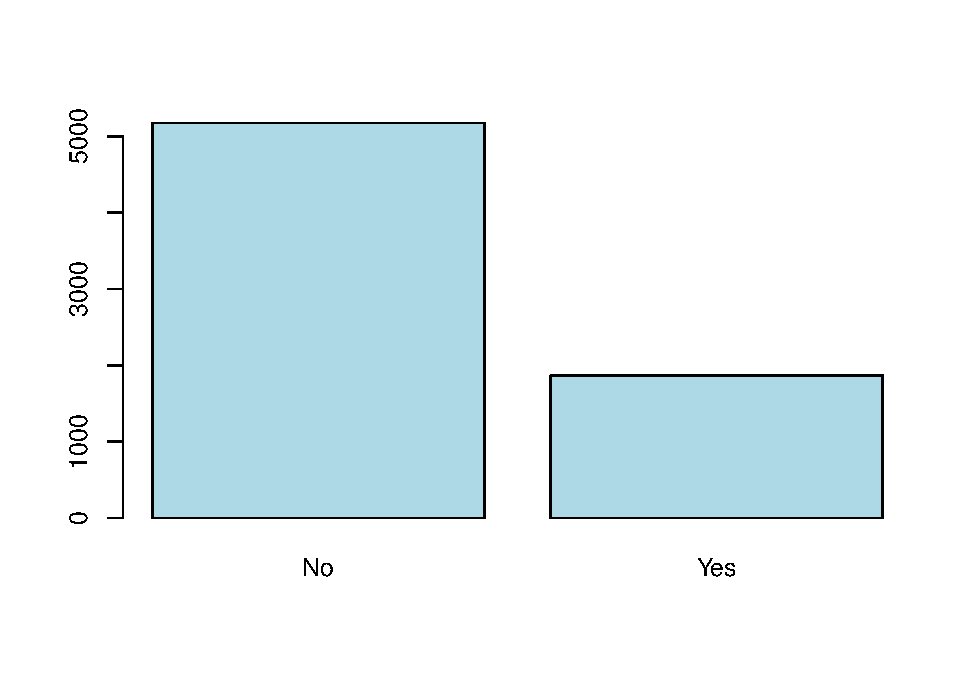
\includegraphics{Assignment2_script_files/figure-latex/unnamed-chunk-25-1.pdf}

\begin{Shaded}
\begin{Highlighting}[]
\CommentTok{\# Mixed Associations (using Chisquared pvalue and CramersV)}
\NormalTok{cat }\OtherTok{\textless{}{-}} \FunctionTok{which}\NormalTok{(}\FunctionTok{sapply}\NormalTok{(df, }\ControlFlowTok{function}\NormalTok{(x) }\FunctionTok{is.factor}\NormalTok{(x) }\SpecialCharTok{||} \FunctionTok{is.character}\NormalTok{(x)))}

\NormalTok{df\_corr }\OtherTok{\textless{}{-}}\NormalTok{ df[,}\SpecialCharTok{{-}}\DecValTok{1}\NormalTok{]}

\CommentTok{\# function to get chi square p value and Cramers V}
\NormalTok{f }\OtherTok{=} \ControlFlowTok{function}\NormalTok{(x,y) \{}
\NormalTok{    tbl }\OtherTok{=}\NormalTok{ df }\SpecialCharTok{\%\textgreater{}\%} \FunctionTok{select}\NormalTok{(x,y) }\SpecialCharTok{\%\textgreater{}\%} \FunctionTok{table}\NormalTok{()}
\NormalTok{    chisq\_pval }\OtherTok{=} \FunctionTok{round}\NormalTok{(}\FunctionTok{chisq.test}\NormalTok{(tbl)}\SpecialCharTok{$}\NormalTok{p.value, }\DecValTok{4}\NormalTok{)}
\NormalTok{    cramV }\OtherTok{=} \FunctionTok{round}\NormalTok{(}\FunctionTok{cramersV}\NormalTok{(tbl), }\DecValTok{4}\NormalTok{) }
    \FunctionTok{data.frame}\NormalTok{(x, y, chisq\_pval, cramV) \}}

\CommentTok{\# create unique combinations of column names}
\CommentTok{\# sorting will help getting a better plot (upper triangular)}
\NormalTok{df\_comb }\OtherTok{=} \FunctionTok{data.frame}\NormalTok{(}\FunctionTok{t}\NormalTok{(}\FunctionTok{combn}\NormalTok{(}\FunctionTok{sort}\NormalTok{(}\FunctionTok{names}\NormalTok{(df\_corr)), }\DecValTok{2}\NormalTok{)), }\AttributeTok{stringsAsFactors =}\NormalTok{ F)}

\CommentTok{\# apply function to each variable combination}
\NormalTok{df\_res }\OtherTok{=} \FunctionTok{map2\_df}\NormalTok{(df\_comb}\SpecialCharTok{$}\NormalTok{X1, df\_comb}\SpecialCharTok{$}\NormalTok{X2, f)}

\CommentTok{\# plot results}
\NormalTok{df\_res }\SpecialCharTok{\%\textgreater{}\%}
  \FunctionTok{ggplot}\NormalTok{(}\FunctionTok{aes}\NormalTok{(x,y,}\AttributeTok{fill=}\NormalTok{chisq\_pval))}\SpecialCharTok{+}
  \FunctionTok{geom\_tile}\NormalTok{()}\SpecialCharTok{+}
  \FunctionTok{geom\_text}\NormalTok{(}\FunctionTok{aes}\NormalTok{(x,y,}\AttributeTok{label=}\NormalTok{cramV), }\AttributeTok{size=}\DecValTok{1}\NormalTok{)}\SpecialCharTok{+}
  \FunctionTok{scale\_fill\_gradient}\NormalTok{(}\AttributeTok{low=}\StringTok{"red"}\NormalTok{, }\AttributeTok{high=}\StringTok{"yellow"}\NormalTok{)}\SpecialCharTok{+}
  \FunctionTok{theme\_classic}\NormalTok{()}\SpecialCharTok{+}
  \FunctionTok{theme}\NormalTok{(}\AttributeTok{axis.text.x =} \FunctionTok{element\_text}\NormalTok{(}\AttributeTok{angle =} \DecValTok{30}\NormalTok{, }\AttributeTok{hjust =} \DecValTok{1}\NormalTok{))}
\end{Highlighting}
\end{Shaded}

\includegraphics{Assignment2_script_files/figure-latex/unnamed-chunk-25-2.pdf}

\begin{Shaded}
\begin{Highlighting}[]
\CommentTok{\# Function to find mixed associations found at:}
\CommentTok{\# https://stackoverflow.com/questions/52554336/plot{-}the{-}equivalent{-}of{-}correlation{-}matrix{-}for{-}factors{-}categorical{-}data{-}and{-}mi}
\CommentTok{\# By AntoniosK on StackOverflow}
\end{Highlighting}
\end{Shaded}

\hypertarget{multivariate-outliers}{%
\section{Multivariate Outliers}\label{multivariate-outliers}}

Using the Moutlier function at a 1\% significance level we find that
there are 62 outliers. Checking the summary of the outliers we see that
they have abnormally high tenure, and very high TotalCharges. However,
when we plot the robust distance versus the mahalanobis distance we see
that there is a lot of continuity in the points. We believe that all the
points so closely together, springing out in three continuous spikes
means that these outliers are expected, as many other observations come
close to this cutoff. Thus, we decide to keep all of the multivariate
outliers. This is becuase of this strong continuity in the graph and the
relatedness of all the points close to the cutoff. Losing these points
mean we lose valuable information as there is a clear pattern, namely
the higher the tenure the higher the overall total charges, even if they
are very high numbers that are shown to be outliers by the Moutlier
function. We want this relationship to be captured in the model.

\begin{Shaded}
\begin{Highlighting}[]
\NormalTok{res.mout }\OtherTok{\textless{}{-}} \FunctionTok{Moutlier}\NormalTok{(df[,num],}\AttributeTok{quantile=}\FloatTok{0.99}\NormalTok{,}\AttributeTok{plot=}\NormalTok{F)}
\FunctionTok{length}\NormalTok{(}\FunctionTok{which}\NormalTok{(res.mout}\SpecialCharTok{$}\NormalTok{md }\SpecialCharTok{\textgreater{}}\NormalTok{ res.mout}\SpecialCharTok{$}\NormalTok{cutoff))}
\end{Highlighting}
\end{Shaded}

\begin{verbatim}
## [1] 62
\end{verbatim}

\begin{Shaded}
\begin{Highlighting}[]
\NormalTok{mout }\OtherTok{\textless{}{-}} \FunctionTok{which}\NormalTok{(res.mout}\SpecialCharTok{$}\NormalTok{md }\SpecialCharTok{\textgreater{}}\NormalTok{ res.mout}\SpecialCharTok{$}\NormalTok{cutoff)}
\FunctionTok{summary}\NormalTok{(df[mout, num]) }\CommentTok{\#Summary of outliers}
\end{Highlighting}
\end{Shaded}

\begin{verbatim}
##      tenure      MonthlyCharges    TotalCharges 
##  Min.   :68.00   Min.   : 19.10   Min.   :1194  
##  1st Qu.:71.00   1st Qu.: 19.70   1st Qu.:1361  
##  Median :71.50   Median : 19.88   Median :1406  
##  Mean   :71.18   Mean   : 21.80   Mean   :1540  
##  3rd Qu.:72.00   3rd Qu.: 20.34   3rd Qu.:1490  
##  Max.   :72.00   Max.   :117.80   Max.   :8685
\end{verbatim}

\begin{Shaded}
\begin{Highlighting}[]
\FunctionTok{plot}\NormalTok{(res.mout}\SpecialCharTok{$}\NormalTok{md, res.mout}\SpecialCharTok{$}\NormalTok{rd)}
\end{Highlighting}
\end{Shaded}

\includegraphics{Assignment2_script_files/figure-latex/unnamed-chunk-26-1.pdf}

\begin{Shaded}
\begin{Highlighting}[]
\CommentTok{\#df \textless{}{-} df[{-}m.out,] \#remove multivariate outliers}
\end{Highlighting}
\end{Shaded}

\hypertarget{modelling}{%
\section{Modelling}\label{modelling}}

Now we enter into the modelling stage of the analysis. We first want to
construct a robust numerical model, in order to add transformations in
the numerical variables. Afterwards we will add the main categorical
variables into this best numerical model, and finally we will look at
interactions between variables to make the final model.

\hypertarget{model-with-numerical-variables}{%
\section{Model with numerical
variables}\label{model-with-numerical-variables}}

We only have 3 numerical variables, so, in the first place, we construct
a model with all 3 numerical variables: tenure, MonthlyCharges and
TotalCharges. We are suspicious of multicolinearity regarding
TotalCharges, since the number calculated by multiplying the tenure
months by MonthlyCharges gives a similar result than the TotalCharges
value (with small a deviation probably coming from opening fees or
discounts in the different contracts).

\begin{Shaded}
\begin{Highlighting}[]
\FunctionTok{attach}\NormalTok{(df)}
\NormalTok{nm1 }\OtherTok{\textless{}{-}} \FunctionTok{glm}\NormalTok{(Churn }\SpecialCharTok{\textasciitilde{}}\NormalTok{ tenure }\SpecialCharTok{+}\NormalTok{ MonthlyCharges }\SpecialCharTok{+}\NormalTok{ TotalCharges, }\AttributeTok{family=}\StringTok{"binomial"}\NormalTok{, }\AttributeTok{data =}\NormalTok{ df)}
\NormalTok{vif.nm1 }\OtherTok{\textless{}{-}} \FunctionTok{vif}\NormalTok{(nm1);vif.nm1}
\end{Highlighting}
\end{Shaded}

\begin{verbatim}
##         tenure MonthlyCharges   TotalCharges 
##      13.650324       2.293852      17.715584
\end{verbatim}

\begin{Shaded}
\begin{Highlighting}[]
\FunctionTok{step}\NormalTok{(nm1,}\AttributeTok{k=} \FunctionTok{log}\NormalTok{(}\FunctionTok{nrow}\NormalTok{(df))) }
\end{Highlighting}
\end{Shaded}

\begin{verbatim}
## Start:  AIC=6424.6
## Churn ~ tenure + MonthlyCharges + TotalCharges
## 
##                  Df Deviance    AIC
## - TotalCharges    1   6394.4 6420.9
## <none>                6389.2 6424.6
## - tenure          1   6576.5 6603.1
## - MonthlyCharges  1   6737.3 6763.8
## 
## Step:  AIC=6420.93
## Churn ~ tenure + MonthlyCharges
## 
##                  Df Deviance    AIC
## <none>                6394.4 6420.9
## - MonthlyCharges  1   7191.9 7209.6
## - tenure          1   7878.2 7895.9
\end{verbatim}

\begin{verbatim}
## 
## Call:  glm(formula = Churn ~ tenure + MonthlyCharges, family = "binomial", 
##     data = df)
## 
## Coefficients:
##    (Intercept)          tenure  MonthlyCharges  
##       -1.80244        -0.05485         0.03295  
## 
## Degrees of Freedom: 7042 Total (i.e. Null);  7040 Residual
## Null Deviance:       8150 
## Residual Deviance: 6394  AIC: 6400
\end{verbatim}

We perform an anova test to see if the variance explained by the two
models is the same

\begin{Shaded}
\begin{Highlighting}[]
\NormalTok{nm2 }\OtherTok{\textless{}{-}} \FunctionTok{glm}\NormalTok{(Churn }\SpecialCharTok{\textasciitilde{}}\NormalTok{ tenure }\SpecialCharTok{+}\NormalTok{ MonthlyCharges, }\AttributeTok{family=}\StringTok{"binomial"}\NormalTok{, }\AttributeTok{data =}\NormalTok{ df)}
\FunctionTok{anova}\NormalTok{(nm2,nm1,}\AttributeTok{test=}\StringTok{"Chisq"}\NormalTok{) }\CommentTok{\#p{-}value: 0.02277 }
\end{Highlighting}
\end{Shaded}

\begin{verbatim}
## Analysis of Deviance Table
## 
## Model 1: Churn ~ tenure + MonthlyCharges
## Model 2: Churn ~ tenure + MonthlyCharges + TotalCharges
##   Resid. Df Resid. Dev Df Deviance Pr(>Chi)  
## 1      7040     6394.4                       
## 2      7039     6389.2  1   5.1862  0.02277 *
## ---
## Signif. codes:  0 '***' 0.001 '**' 0.01 '*' 0.05 '.' 0.1 ' ' 1
\end{verbatim}

Since the p-value is 0.02277, at 99\% confidence we do not reject and
accept the simple model as the best one.

\hypertarget{transformations-of-numerical-variables}{%
\section{Transformations of numerical
variables}\label{transformations-of-numerical-variables}}

Firstly, we examine marginalModelPlots to gain insights into which
variables effectively fit the model. Subsequently, we observed the
necessity for a transformation in the tenure variable. A reduction of
one unit in tenure is associated with a log-odds increase of -0.054850
for Churn. Consequently, implementing a Square Root Transformation
becomes imperative.

\begin{Shaded}
\begin{Highlighting}[]
\NormalTok{nm3 }\OtherTok{\textless{}{-}} \FunctionTok{glm}\NormalTok{(Churn }\SpecialCharTok{\textasciitilde{}}\NormalTok{ tenure}\SpecialCharTok{+} \FunctionTok{I}\NormalTok{(tenure}\SpecialCharTok{\^{}}\DecValTok{2}\NormalTok{) }\SpecialCharTok{+}\NormalTok{ MonthlyCharges, }\AttributeTok{family=}\StringTok{"binomial"}\NormalTok{, }\AttributeTok{data =}\NormalTok{ df)}
\FunctionTok{marginalModelPlots}\NormalTok{(nm3)}
\end{Highlighting}
\end{Shaded}

\includegraphics{Assignment2_script_files/figure-latex/unnamed-chunk-29-1.pdf}

\begin{Shaded}
\begin{Highlighting}[]
\NormalTok{nm4 }\OtherTok{\textless{}{-}} \FunctionTok{glm}\NormalTok{(Churn }\SpecialCharTok{\textasciitilde{}} \FunctionTok{poly}\NormalTok{(tenure,}\DecValTok{2}\NormalTok{) }\SpecialCharTok{+}\NormalTok{ MonthlyCharges, }\AttributeTok{family=}\StringTok{"binomial"}\NormalTok{, }\AttributeTok{data =}\NormalTok{ df)}
\FunctionTok{marginalModelPlots}\NormalTok{(nm4)}
\end{Highlighting}
\end{Shaded}

\includegraphics{Assignment2_script_files/figure-latex/unnamed-chunk-29-2.pdf}

\hypertarget{nm4-residual-analysis-and-influential-data}{%
\section{NM4: Residual analysis and Influential
Data}\label{nm4-residual-analysis-and-influential-data}}

(INTERPRETATION OF RESIDUAL PLOTS)

When looking at the hat values, using the influenceIndexPlot, we see
that there are many no points that stand out relative to the rest. We
have a similar case when looking at the influencePlot. We can confirm
that there are no outstanding hat values by drawing a boxplot and a
typical cutoff line at 4*p/n.~This plot shows us there are no points
with hat values above this cutoff and therefore no further action needs
to be taken.

In a similar way, when we plot the influenceIndexPlot for Cooks'
Distance, we find a few (approximately 5) points that stand out above
the rest. To further investigate we draw a boxplot of Cooks' Distance
and find that indeed there are four points that are relatively further
out than others. We can draw a clear cutoff line at 0.003 to separate
these points. When we further inspect these points by comparing their
summary statistics against overall summaries of Tenure and Monthly
Charges we find that tenure is significantly higher for these outlier
observations while the average MonthlyCharges are almost half of the
overall average. We decide to remove these points.

\begin{Shaded}
\begin{Highlighting}[]
\CommentTok{\# Residuals}
\FunctionTok{residualPlots}\NormalTok{(nm4, }\AttributeTok{layout=}\FunctionTok{c}\NormalTok{(}\DecValTok{1}\NormalTok{, }\DecValTok{3}\NormalTok{))}
\end{Highlighting}
\end{Shaded}

\includegraphics{Assignment2_script_files/figure-latex/unnamed-chunk-30-1.pdf}

\begin{verbatim}
##                 Test stat Pr(>|Test stat|)
## poly(tenure, 2)                           
## MonthlyCharges     0.0255           0.8732
\end{verbatim}

\begin{Shaded}
\begin{Highlighting}[]
\FunctionTok{influencePlot}\NormalTok{(nm4)}
\end{Highlighting}
\end{Shaded}

\includegraphics{Assignment2_script_files/figure-latex/unnamed-chunk-30-2.pdf}

\begin{verbatim}
##         StudRes          Hat        CookD
## 269   2.9660363 0.0001596978 0.0031880647
## 431   2.9893903 0.0001567313 0.0033558372
## 4587 -0.6462575 0.0018793961 0.0001093968
## 6119 -0.6408873 0.0018510422 0.0001057701
## 6425  2.7056019 0.0003598658 0.0033855901
\end{verbatim}

\begin{Shaded}
\begin{Highlighting}[]
\CommentTok{\# Hat values}
\FunctionTok{influenceIndexPlot}\NormalTok{(nm4, }\AttributeTok{id.n=}\DecValTok{10}\NormalTok{, }\AttributeTok{vars=}\FunctionTok{c}\NormalTok{(}\StringTok{\textquotesingle{}hat\textquotesingle{}}\NormalTok{))}
\end{Highlighting}
\end{Shaded}

\includegraphics{Assignment2_script_files/figure-latex/unnamed-chunk-30-3.pdf}

\begin{Shaded}
\begin{Highlighting}[]
\FunctionTok{Boxplot}\NormalTok{(}\FunctionTok{hatvalues}\NormalTok{(nm4), }\AttributeTok{ylim=}\FunctionTok{c}\NormalTok{(}\DecValTok{0}\NormalTok{,}\FloatTok{0.0025}\NormalTok{))}
\end{Highlighting}
\end{Shaded}

\begin{verbatim}
##  [1] 4587 6119 4611 3206 6769 4156 2369 5348 2026 4207
\end{verbatim}

\begin{Shaded}
\begin{Highlighting}[]
\FunctionTok{abline}\NormalTok{(}\AttributeTok{h=}\DecValTok{4}\SpecialCharTok{*}\FunctionTok{length}\NormalTok{(}\FunctionTok{coef}\NormalTok{(nm4))}\SpecialCharTok{/}\FunctionTok{nrow}\NormalTok{(df))}
\end{Highlighting}
\end{Shaded}

\includegraphics{Assignment2_script_files/figure-latex/unnamed-chunk-30-4.pdf}

\begin{Shaded}
\begin{Highlighting}[]
\CommentTok{\# Cooks distance}
\FunctionTok{influenceIndexPlot}\NormalTok{(nm4, }\AttributeTok{id.n=}\DecValTok{10}\NormalTok{, }\AttributeTok{vars=}\FunctionTok{c}\NormalTok{(}\StringTok{\textquotesingle{}Cook\textquotesingle{}}\NormalTok{))}
\end{Highlighting}
\end{Shaded}

\includegraphics{Assignment2_script_files/figure-latex/unnamed-chunk-30-5.pdf}

\begin{Shaded}
\begin{Highlighting}[]
\FunctionTok{Boxplot}\NormalTok{(}\FunctionTok{cooks.distance}\NormalTok{(nm4))}
\end{Highlighting}
\end{Shaded}

\begin{verbatim}
##  [1] 6425  431 4150 5842  269 4820 4796 6793 4273 5087
\end{verbatim}

\begin{Shaded}
\begin{Highlighting}[]
\FunctionTok{abline}\NormalTok{(}\AttributeTok{h=}\FloatTok{0.003}\NormalTok{)}
\end{Highlighting}
\end{Shaded}

\includegraphics{Assignment2_script_files/figure-latex/unnamed-chunk-30-6.pdf}

\begin{Shaded}
\begin{Highlighting}[]
\NormalTok{llcoo }\OtherTok{\textless{}{-}} \FunctionTok{which}\NormalTok{(}\FunctionTok{cooks.distance}\NormalTok{(nm4)}\SpecialCharTok{\textgreater{}} \FloatTok{0.003}\NormalTok{);}
\FunctionTok{summary}\NormalTok{(df[,}\FunctionTok{c}\NormalTok{(}\StringTok{\textquotesingle{}tenure\textquotesingle{}}\NormalTok{, }\StringTok{\textquotesingle{}MonthlyCharges\textquotesingle{}}\NormalTok{)])}
\end{Highlighting}
\end{Shaded}

\begin{verbatim}
##      tenure      MonthlyCharges  
##  Min.   : 0.00   Min.   : 18.25  
##  1st Qu.: 9.00   1st Qu.: 35.50  
##  Median :29.00   Median : 70.35  
##  Mean   :32.37   Mean   : 64.76  
##  3rd Qu.:55.00   3rd Qu.: 89.85  
##  Max.   :72.00   Max.   :118.75
\end{verbatim}

\begin{Shaded}
\begin{Highlighting}[]
\FunctionTok{summary}\NormalTok{(df[llcoo,}\FunctionTok{c}\NormalTok{(}\StringTok{\textquotesingle{}tenure\textquotesingle{}}\NormalTok{, }\StringTok{\textquotesingle{}MonthlyCharges\textquotesingle{}}\NormalTok{)])}
\end{Highlighting}
\end{Shaded}

\begin{verbatim}
##      tenure     MonthlyCharges 
##  Min.   :59.0   Min.   :19.35  
##  1st Qu.:61.0   1st Qu.:19.40  
##  Median :70.0   Median :45.25  
##  Mean   :66.6   Mean   :37.51  
##  3rd Qu.:71.0   3rd Qu.:49.35  
##  Max.   :72.0   Max.   :54.20
\end{verbatim}

\begin{Shaded}
\begin{Highlighting}[]
\NormalTok{df }\OtherTok{\textless{}{-}}\NormalTok{ df[}\SpecialCharTok{{-}}\NormalTok{llcoo,]}
\FunctionTok{rownames}\NormalTok{(df) }\OtherTok{\textless{}{-}} \ConstantTok{NULL}
\end{Highlighting}
\end{Shaded}

\hypertarget{adding-main-categorical-effects}{%
\section{Adding main categorical
effects}\label{adding-main-categorical-effects}}

Now we attempt to add our factor variables to the model. First we are
building an inicial model with the main numerical variables and all the
categorical ones, which will obviously result in a too complex model to
be analysed or properly interpreted. After that, we are conducting an
Anova Chisq test to assess the significance of each categorical
variable.

\begin{Shaded}
\begin{Highlighting}[]
\NormalTok{cm1 }\OtherTok{\textless{}{-}} \FunctionTok{glm}\NormalTok{(Churn }\SpecialCharTok{\textasciitilde{}} \FunctionTok{poly}\NormalTok{(tenure,}\DecValTok{2}\NormalTok{) }\SpecialCharTok{+}\NormalTok{ MonthlyCharges }\SpecialCharTok{+}\NormalTok{ gender }\SpecialCharTok{+}\NormalTok{ SeniorCitizen }\SpecialCharTok{+}\NormalTok{ Partner }\SpecialCharTok{+}\NormalTok{ Dependents }\SpecialCharTok{+}\NormalTok{ PhoneService }\SpecialCharTok{+}\NormalTok{ MultipleLines }\SpecialCharTok{+}\NormalTok{ InternetService }\SpecialCharTok{+}\NormalTok{ OnlineSecurity }\SpecialCharTok{+}\NormalTok{ OnlineBackup }\SpecialCharTok{+}\NormalTok{ DeviceProtection }\SpecialCharTok{+}\NormalTok{ TechSupport }\SpecialCharTok{+}\NormalTok{ StreamingTV }\SpecialCharTok{+}\NormalTok{ StreamingMovies }\SpecialCharTok{+}\NormalTok{ Contract }\SpecialCharTok{+}\NormalTok{ PaperlessBilling }\SpecialCharTok{+}\NormalTok{ PaymentMethod, }\AttributeTok{family=}\StringTok{"binomial"}\NormalTok{, }\AttributeTok{data =}\NormalTok{ df)}
\FunctionTok{Anova}\NormalTok{(cm1,}\AttributeTok{test=}\StringTok{"LR"}\NormalTok{)}
\end{Highlighting}
\end{Shaded}

\begin{verbatim}
## Analysis of Deviance Table (Type II tests)
## 
## Response: Churn
##                  LR Chisq Df Pr(>Chisq)    
## poly(tenure, 2)   295.599  2  < 2.2e-16 ***
## MonthlyCharges      0.910  1   0.339996    
## gender              0.100  1   0.751910    
## SeniorCitizen       7.125  1   0.007602 ** 
## Partner             0.004  1   0.950749    
## Dependents          2.063  1   0.150926    
## PhoneService               0               
## MultipleLines       7.968  1   0.004762 ** 
## InternetService     4.411  1   0.035699 *  
## OnlineSecurity      1.006  1   0.315820    
## OnlineBackup        0.012  1   0.913028    
## DeviceProtection    0.977  1   0.322887    
## TechSupport         0.562  1   0.453597    
## StreamingTV         3.263  1   0.070872 .  
## StreamingMovies     3.347  1   0.067312 .  
## Contract          120.396  2  < 2.2e-16 ***
## PaperlessBilling   20.170  1  7.087e-06 ***
## PaymentMethod      22.268  3  5.738e-05 ***
## ---
## Signif. codes:  0 '***' 0.001 '**' 0.01 '*' 0.05 '.' 0.1 ' ' 1
\end{verbatim}

This Anova tests suggests, at 95\% confidence, to take out of the
modeling the following variables: gender, Partner, Dependets,
PhoneService, OnlineSecurity, OnlineBackup, DeviceProtection,
TechSupport, StreamingTV and StreamingMovies. Now we construct a model
only with the significant variables.

\begin{Shaded}
\begin{Highlighting}[]
\NormalTok{cm2 }\OtherTok{\textless{}{-}} \FunctionTok{glm}\NormalTok{(Churn }\SpecialCharTok{\textasciitilde{}} \FunctionTok{poly}\NormalTok{(tenure,}\DecValTok{2}\NormalTok{) }\SpecialCharTok{+}\NormalTok{ MonthlyCharges }\SpecialCharTok{+}\NormalTok{ SeniorCitizen }\SpecialCharTok{+}\NormalTok{ MultipleLines }\SpecialCharTok{+}\NormalTok{ InternetService }\SpecialCharTok{+}\NormalTok{ Contract }\SpecialCharTok{+}\NormalTok{ PaperlessBilling }\SpecialCharTok{+}\NormalTok{ PaymentMethod, }\AttributeTok{family=}\StringTok{"binomial"}\NormalTok{, }\AttributeTok{data =}\NormalTok{ df)}
\end{Highlighting}
\end{Shaded}

\hypertarget{cm2-residual-analysis-and-influential-data}{%
\section{CM2: Residual Analysis and Influential
Data}\label{cm2-residual-analysis-and-influential-data}}

(INTERPRETATION OF RESIDUAL PLOTS)

From the general influencePlot we can see that there are a couple
possible outliers that need further investivation such as observations
3821 and 489, which seem to have abnormally high hat values. These same
points stand out in the influenceIndexPlot. When we now draw a boxplot
of the hat values and draw a cutoff line at the typical cutoff 4*p/n, we
see that point 489 is the only one above this cutoff, with point 2819
just below. Thus, we remove observation 489.

When we further investigate Cooks' Distance using influenceIndexPlot we
see more observations stand out with observations 3972 and 5948 being
fat above the rest. Now when we draw the boxplot, we again see these two
points stand out with several other points. Here there is no clear
cutoff as the observations splinter into groups, where one group has a
large distance to the rest, and then the two observations mentioned even
further than this. Thus, to not lose too much valuable information we
decide to remove only the two largest outliers, thus moving the cutoff
to 0.0033. When comparing the Cooks outliers summaries to the all the
data it is difficult to see where they are different. They seem to
generally have lower charges (monthly and total), with longer tenure but
nothing noteworthy that would suggest why they seem to be so influential
from the summary statistics alone.

\begin{Shaded}
\begin{Highlighting}[]
\CommentTok{\# Residuals}
\FunctionTok{residualPlots}\NormalTok{(cm2, }\AttributeTok{layout=}\FunctionTok{c}\NormalTok{(}\DecValTok{1}\NormalTok{, }\DecValTok{3}\NormalTok{))}
\end{Highlighting}
\end{Shaded}

\includegraphics{Assignment2_script_files/figure-latex/unnamed-chunk-33-1.pdf}
\includegraphics{Assignment2_script_files/figure-latex/unnamed-chunk-33-2.pdf}
\includegraphics{Assignment2_script_files/figure-latex/unnamed-chunk-33-3.pdf}

\begin{verbatim}
##                  Test stat Pr(>|Test stat|)   
## poly(tenure, 2)                               
## MonthlyCharges      6.7304         0.009479 **
## SeniorCitizen                                 
## MultipleLines                                 
## InternetService                               
## Contract                                      
## PaperlessBilling                              
## PaymentMethod                                 
## ---
## Signif. codes:  0 '***' 0.001 '**' 0.01 '*' 0.05 '.' 0.1 ' ' 1
\end{verbatim}

\begin{Shaded}
\begin{Highlighting}[]
\FunctionTok{influencePlot}\NormalTok{(cm2)}
\end{Highlighting}
\end{Shaded}

\includegraphics{Assignment2_script_files/figure-latex/unnamed-chunk-33-4.pdf}

\begin{verbatim}
##         StudRes          Hat        CookD
## 487  -0.6808226 0.0087949451 0.0001547851
## 3819 -1.0230782 0.0080644712 0.0003731883
## 3970  3.0140048 0.0006158875 0.0037127146
## 4270  3.1328757 0.0003653224 0.0031950636
## 4817  3.3328830 0.0001889194 0.0031652752
## 5944  3.0000940 0.0006272134 0.0036268210
\end{verbatim}

\begin{Shaded}
\begin{Highlighting}[]
\CommentTok{\# Hat values}
\FunctionTok{influenceIndexPlot}\NormalTok{(cm2, }\AttributeTok{id.n=}\DecValTok{10}\NormalTok{, }\AttributeTok{vars=}\FunctionTok{c}\NormalTok{(}\StringTok{\textquotesingle{}hat\textquotesingle{}}\NormalTok{))}
\end{Highlighting}
\end{Shaded}

\includegraphics{Assignment2_script_files/figure-latex/unnamed-chunk-33-5.pdf}

\begin{Shaded}
\begin{Highlighting}[]
\FunctionTok{Boxplot}\NormalTok{(}\FunctionTok{hatvalues}\NormalTok{(cm2), }\AttributeTok{ylim=}\FunctionTok{c}\NormalTok{(}\DecValTok{0}\NormalTok{,}\FloatTok{0.01}\NormalTok{))}
\end{Highlighting}
\end{Shaded}

\begin{verbatim}
##  [1]  487 3819 5012 5700 4336 1339 2897 5896 4335 4695
\end{verbatim}

\begin{Shaded}
\begin{Highlighting}[]
\FunctionTok{abline}\NormalTok{(}\AttributeTok{h=}\DecValTok{4}\SpecialCharTok{*}\FunctionTok{length}\NormalTok{(}\FunctionTok{coef}\NormalTok{(cm2))}\SpecialCharTok{/}\FunctionTok{nrow}\NormalTok{(df))}
\end{Highlighting}
\end{Shaded}

\includegraphics{Assignment2_script_files/figure-latex/unnamed-chunk-33-6.pdf}

\begin{Shaded}
\begin{Highlighting}[]
\CommentTok{\# hatvalues(cm2)[487] {-}{-}\textgreater{} referring to observation 489}
\NormalTok{df }\OtherTok{\textless{}{-}}\NormalTok{ df[}\SpecialCharTok{{-}}\DecValTok{489}\NormalTok{,]}
\FunctionTok{rownames}\NormalTok{(df) }\OtherTok{\textless{}{-}} \ConstantTok{NULL}

\CommentTok{\# Cooks distance}
\FunctionTok{influenceIndexPlot}\NormalTok{(cm2, }\AttributeTok{id.n=}\DecValTok{10}\NormalTok{, }\AttributeTok{vars=}\FunctionTok{c}\NormalTok{(}\StringTok{\textquotesingle{}Cook\textquotesingle{}}\NormalTok{))}
\end{Highlighting}
\end{Shaded}

\includegraphics{Assignment2_script_files/figure-latex/unnamed-chunk-33-7.pdf}

\begin{Shaded}
\begin{Highlighting}[]
\FunctionTok{Boxplot}\NormalTok{(}\FunctionTok{cooks.distance}\NormalTok{(cm2))}
\end{Highlighting}
\end{Shaded}

\begin{verbatim}
##  [1] 3970 5944 4270 4817 5587 4511 6720 4525 6676 3778
\end{verbatim}

\begin{Shaded}
\begin{Highlighting}[]
\FunctionTok{abline}\NormalTok{(}\AttributeTok{h=}\FloatTok{0.0033}\NormalTok{)}
\end{Highlighting}
\end{Shaded}

\includegraphics{Assignment2_script_files/figure-latex/unnamed-chunk-33-8.pdf}

\begin{Shaded}
\begin{Highlighting}[]
\NormalTok{llcoo }\OtherTok{\textless{}{-}} \FunctionTok{which}\NormalTok{(}\FunctionTok{cooks.distance}\NormalTok{(cm2)}\SpecialCharTok{\textgreater{}} \FloatTok{0.0033}\NormalTok{);}
\CommentTok{\#summary(df)          {-}{-}\textgreater{} uncomment to compare}
\CommentTok{\#summary(df[llcoo,])  {-}{-}\textgreater{} uncomment to compare}

\NormalTok{df }\OtherTok{\textless{}{-}}\NormalTok{ df[}\SpecialCharTok{{-}}\NormalTok{llcoo,]}
\FunctionTok{rownames}\NormalTok{(df) }\OtherTok{\textless{}{-}} \ConstantTok{NULL}
\end{Highlighting}
\end{Shaded}

\begin{Shaded}
\begin{Highlighting}[]
\NormalTok{cm2 }\OtherTok{\textless{}{-}} \FunctionTok{glm}\NormalTok{(Churn }\SpecialCharTok{\textasciitilde{}} \FunctionTok{poly}\NormalTok{(tenure,}\DecValTok{2}\NormalTok{) }\SpecialCharTok{+}\NormalTok{ MonthlyCharges }\SpecialCharTok{+}\NormalTok{ SeniorCitizen }\SpecialCharTok{+}\NormalTok{ MultipleLines }\SpecialCharTok{+}\NormalTok{ InternetService }\SpecialCharTok{+}\NormalTok{ Contract }\SpecialCharTok{+}\NormalTok{ PaperlessBilling }\SpecialCharTok{+}\NormalTok{ PaymentMethod, }\AttributeTok{family=}\StringTok{"binomial"}\NormalTok{, }\AttributeTok{data =}\NormalTok{ df)}
\end{Highlighting}
\end{Shaded}

\hypertarget{interactions}{%
\section{Interactions}\label{interactions}}

Significant interactions (5\% level):\\
poly(tenure, 2):Contract\\
MonthlyCharges:MultipleLines\\
MonthlyCharges:InternetService\\
MonthlyCharges:Contract\\
SeniorCitizen:PaymentMethod\\
InternetService:Contract\\
InternetService:PaymentMethod

\begin{Shaded}
\begin{Highlighting}[]
\FunctionTok{Anova}\NormalTok{(}\FunctionTok{glm}\NormalTok{(Churn }\SpecialCharTok{\textasciitilde{}}\NormalTok{ (}\FunctionTok{poly}\NormalTok{(tenure,}\DecValTok{2}\NormalTok{) }\SpecialCharTok{+}\NormalTok{ MonthlyCharges }\SpecialCharTok{+}\NormalTok{ SeniorCitizen }\SpecialCharTok{+}\NormalTok{ MultipleLines }\SpecialCharTok{+}\NormalTok{ InternetService }\SpecialCharTok{+}\NormalTok{ Contract }\SpecialCharTok{+}\NormalTok{ PaperlessBilling }\SpecialCharTok{+}\NormalTok{ PaymentMethod) }\SpecialCharTok{*}\NormalTok{ (}\FunctionTok{poly}\NormalTok{(tenure,}\DecValTok{2}\NormalTok{) }\SpecialCharTok{+}\NormalTok{ MonthlyCharges }\SpecialCharTok{+}\NormalTok{ SeniorCitizen }\SpecialCharTok{+}\NormalTok{ MultipleLines }\SpecialCharTok{+}\NormalTok{ InternetService }\SpecialCharTok{+}\NormalTok{ Contract }\SpecialCharTok{+}\NormalTok{ PaperlessBilling }\SpecialCharTok{+}\NormalTok{ PaymentMethod), }\AttributeTok{family=}\StringTok{"binomial"}\NormalTok{, }\AttributeTok{data =}\NormalTok{ df))}
\end{Highlighting}
\end{Shaded}

\begin{verbatim}
## Analysis of Deviance Table (Type II tests)
## 
## Response: Churn
##                                  LR Chisq Df Pr(>Chisq)    
## poly(tenure, 2)                    353.01  2  < 2.2e-16 ***
## MonthlyCharges                       8.47  1  0.0036015 ** 
## SeniorCitizen                        9.38  1  0.0021979 ** 
## MultipleLines                       18.01  2  0.0001228 ***
## InternetService                     40.35  2  1.727e-09 ***
## Contract                           114.48  2  < 2.2e-16 ***
## PaperlessBilling                    24.49  1  7.487e-07 ***
## PaymentMethod                       31.75  3  5.896e-07 ***
## poly(tenure, 2):MonthlyCharges       1.16  2  0.5588909    
## poly(tenure, 2):SeniorCitizen        2.39  2  0.3032295    
## poly(tenure, 2):MultipleLines        0.53  4  0.9701025    
## poly(tenure, 2):InternetService      2.35  4  0.6721362    
## poly(tenure, 2):Contract            22.56  4  0.0001547 ***
## poly(tenure, 2):PaperlessBilling     5.34  2  0.0693936 .  
## poly(tenure, 2):PaymentMethod       14.00  6  0.0296045 *  
## MonthlyCharges:SeniorCitizen         0.06  1  0.8083933    
## MonthlyCharges:MultipleLines         7.67  2  0.0216087 *  
## MonthlyCharges:InternetService      16.11  2  0.0003172 ***
## MonthlyCharges:Contract             12.63  2  0.0018079 ** 
## MonthlyCharges:PaperlessBilling      0.08  1  0.7748776    
## MonthlyCharges:PaymentMethod         4.96  3  0.1746787    
## SeniorCitizen:MultipleLines          1.89  2  0.3885162    
## SeniorCitizen:InternetService        0.29  2  0.8646871    
## SeniorCitizen:Contract               2.00  2  0.3686318    
## SeniorCitizen:PaperlessBilling       0.01  1  0.9284968    
## SeniorCitizen:PaymentMethod         12.34  3  0.0062953 ** 
## MultipleLines:InternetService        1.07  2  0.5865189    
## MultipleLines:Contract               8.58  4  0.0723792 .  
## MultipleLines:PaperlessBilling       2.05  2  0.3580582    
## MultipleLines:PaymentMethod          6.48  6  0.3715010    
## InternetService:Contract            18.44  4  0.0010127 ** 
## InternetService:PaperlessBilling     1.02  2  0.6010553    
## InternetService:PaymentMethod       18.44  6  0.0052278 ** 
## Contract:PaperlessBilling            3.46  2  0.1770413    
## Contract:PaymentMethod               4.94  6  0.5512889    
## PaperlessBilling:PaymentMethod       2.76  3  0.4300596    
## ---
## Signif. codes:  0 '***' 0.001 '**' 0.01 '*' 0.05 '.' 0.1 ' ' 1
\end{verbatim}

We will be adding interactions one by one to our model, and we will see
if they have significance over the last model, and, if they do, we keep
them in the model and move on. Note that to do that we will be using
Fisher tests, with the null hypothesis being that the variance explained
by both models are the same.\\
First we look into the interaction between Contract and the transformed
tenure. We can see that the role it performs on the model is to \ldots{}
. Then, we perform an Fisher test to see if the variances explained by
the two models are the same or not.

\begin{Shaded}
\begin{Highlighting}[]
\NormalTok{gm1 }\OtherTok{\textless{}{-}} \FunctionTok{glm}\NormalTok{(Churn }\SpecialCharTok{\textasciitilde{}} \FunctionTok{poly}\NormalTok{(tenure,}\DecValTok{2}\NormalTok{)}\SpecialCharTok{*}\NormalTok{Contract }\SpecialCharTok{+}\NormalTok{ MonthlyCharges }\SpecialCharTok{+}\NormalTok{ SeniorCitizen }\SpecialCharTok{+}\NormalTok{ MultipleLines }\SpecialCharTok{+}\NormalTok{ InternetService }\SpecialCharTok{+}\NormalTok{ PaperlessBilling }\SpecialCharTok{+}\NormalTok{ PaymentMethod, }\AttributeTok{family=}\StringTok{"binomial"}\NormalTok{, }\AttributeTok{data =}\NormalTok{ df)}
\FunctionTok{anova}\NormalTok{(cm2,gm1,}\AttributeTok{test=}\StringTok{"Chisq"}\NormalTok{) }\CommentTok{\#p{-}value 2.982e{-}06}
\end{Highlighting}
\end{Shaded}

\begin{verbatim}
## Analysis of Deviance Table
## 
## Model 1: Churn ~ poly(tenure, 2) + MonthlyCharges + SeniorCitizen + MultipleLines + 
##     InternetService + Contract + PaperlessBilling + PaymentMethod
## Model 2: Churn ~ poly(tenure, 2) * Contract + MonthlyCharges + SeniorCitizen + 
##     MultipleLines + InternetService + PaperlessBilling + PaymentMethod
##   Resid. Df Resid. Dev Df Deviance  Pr(>Chi)    
## 1      7020     5819.4                          
## 2      7016     5788.4  4   31.056 2.982e-06 ***
## ---
## Signif. codes:  0 '***' 0.001 '**' 0.01 '*' 0.05 '.' 0.1 ' ' 1
\end{verbatim}

We can see that the p-value in this case is 2.982e-06, so we reject the
null hypothesis and we decide to keep the interaction forward. Now let's
look at the interactions regarding MonthlyCharges, starting by its
interaction with MultipleLines.

\begin{Shaded}
\begin{Highlighting}[]
\NormalTok{gm2 }\OtherTok{\textless{}{-}} \FunctionTok{glm}\NormalTok{(Churn }\SpecialCharTok{\textasciitilde{}} \FunctionTok{poly}\NormalTok{(tenure,}\DecValTok{2}\NormalTok{)}\SpecialCharTok{*}\NormalTok{Contract }\SpecialCharTok{+}\NormalTok{ MonthlyCharges}\SpecialCharTok{*}\NormalTok{MultipleLines }\SpecialCharTok{+}\NormalTok{ SeniorCitizen }\SpecialCharTok{+}\NormalTok{ MultipleLines }\SpecialCharTok{+}\NormalTok{ InternetService }\SpecialCharTok{+}\NormalTok{ PaperlessBilling }\SpecialCharTok{+}\NormalTok{ PaymentMethod, }\AttributeTok{family=}\StringTok{"binomial"}\NormalTok{, }\AttributeTok{data =}\NormalTok{ df)}
\FunctionTok{anova}\NormalTok{(gm1,gm2,}\AttributeTok{test=}\StringTok{"Chisq"}\NormalTok{) }\CommentTok{\#p{-}value 0.01424 }
\end{Highlighting}
\end{Shaded}

\begin{verbatim}
## Analysis of Deviance Table
## 
## Model 1: Churn ~ poly(tenure, 2) * Contract + MonthlyCharges + SeniorCitizen + 
##     MultipleLines + InternetService + PaperlessBilling + PaymentMethod
## Model 2: Churn ~ poly(tenure, 2) * Contract + MonthlyCharges * MultipleLines + 
##     SeniorCitizen + MultipleLines + InternetService + PaperlessBilling + 
##     PaymentMethod
##   Resid. Df Resid. Dev Df Deviance Pr(>Chi)  
## 1      7016     5788.4                       
## 2      7014     5779.9  2   8.5034  0.01424 *
## ---
## Signif. codes:  0 '***' 0.001 '**' 0.01 '*' 0.05 '.' 0.1 ' ' 1
\end{verbatim}

In this case, the p-value is 0.01424, which would make us reject the
hypothesis at 99\% confidence, but accept it at 95\%. We decide to take
it out of the model.

\begin{Shaded}
\begin{Highlighting}[]
\NormalTok{gm3 }\OtherTok{\textless{}{-}} \FunctionTok{glm}\NormalTok{(Churn }\SpecialCharTok{\textasciitilde{}} \FunctionTok{poly}\NormalTok{(tenure,}\DecValTok{2}\NormalTok{)}\SpecialCharTok{*}\NormalTok{Contract }\SpecialCharTok{+}\NormalTok{ MonthlyCharges}\SpecialCharTok{*}\NormalTok{InternetService }\SpecialCharTok{+}\NormalTok{ SeniorCitizen }\SpecialCharTok{+}\NormalTok{ MultipleLines }\SpecialCharTok{+}\NormalTok{ InternetService }\SpecialCharTok{+}\NormalTok{ PaperlessBilling }\SpecialCharTok{+}\NormalTok{ PaymentMethod, }\AttributeTok{family=}\StringTok{"binomial"}\NormalTok{, }\AttributeTok{data =}\NormalTok{ df)}
\FunctionTok{anova}\NormalTok{(gm1,gm3,}\AttributeTok{test=}\StringTok{"Chisq"}\NormalTok{) }\CommentTok{\#p{-}value 0.005535  }
\end{Highlighting}
\end{Shaded}

\begin{verbatim}
## Analysis of Deviance Table
## 
## Model 1: Churn ~ poly(tenure, 2) * Contract + MonthlyCharges + SeniorCitizen + 
##     MultipleLines + InternetService + PaperlessBilling + PaymentMethod
## Model 2: Churn ~ poly(tenure, 2) * Contract + MonthlyCharges * InternetService + 
##     SeniorCitizen + MultipleLines + InternetService + PaperlessBilling + 
##     PaymentMethod
##   Resid. Df Resid. Dev Df Deviance Pr(>Chi)   
## 1      7016     5788.4                        
## 2      7014     5778.0  2   10.393 0.005535 **
## ---
## Signif. codes:  0 '***' 0.001 '**' 0.01 '*' 0.05 '.' 0.1 ' ' 1
\end{verbatim}

This time, the p-value is 0.005535, so we will keep the interaction in
the model.

\begin{Shaded}
\begin{Highlighting}[]
\NormalTok{gm4 }\OtherTok{\textless{}{-}} \FunctionTok{glm}\NormalTok{(Churn }\SpecialCharTok{\textasciitilde{}} \FunctionTok{poly}\NormalTok{(tenure,}\DecValTok{2}\NormalTok{)}\SpecialCharTok{*}\NormalTok{Contract }\SpecialCharTok{+}\NormalTok{ MonthlyCharges}\SpecialCharTok{*}\NormalTok{(InternetService }\SpecialCharTok{+}\NormalTok{ Contract) }\SpecialCharTok{+}\NormalTok{ SeniorCitizen }\SpecialCharTok{+}\NormalTok{ MultipleLines }\SpecialCharTok{+}\NormalTok{ InternetService }\SpecialCharTok{+}\NormalTok{ PaperlessBilling }\SpecialCharTok{+}\NormalTok{ PaymentMethod, }\AttributeTok{family=}\StringTok{"binomial"}\NormalTok{, }\AttributeTok{data =}\NormalTok{ df)}
\FunctionTok{anova}\NormalTok{(gm3,gm4,}\AttributeTok{test=}\StringTok{"Chisq"}\NormalTok{) }\CommentTok{\#p{-}value 0.8 }
\end{Highlighting}
\end{Shaded}

\begin{verbatim}
## Analysis of Deviance Table
## 
## Model 1: Churn ~ poly(tenure, 2) * Contract + MonthlyCharges * InternetService + 
##     SeniorCitizen + MultipleLines + InternetService + PaperlessBilling + 
##     PaymentMethod
## Model 2: Churn ~ poly(tenure, 2) * Contract + MonthlyCharges * (InternetService + 
##     Contract) + SeniorCitizen + MultipleLines + InternetService + 
##     PaperlessBilling + PaymentMethod
##   Resid. Df Resid. Dev Df Deviance Pr(>Chi)
## 1      7014     5778.0                     
## 2      7012     5777.5  2   0.4462      0.8
\end{verbatim}

Now the p-value is 0.8, so we accept the null hypothesis and not keep
this interaction.

\begin{Shaded}
\begin{Highlighting}[]
\NormalTok{gm5 }\OtherTok{\textless{}{-}} \FunctionTok{glm}\NormalTok{(Churn }\SpecialCharTok{\textasciitilde{}} \FunctionTok{poly}\NormalTok{(tenure,}\DecValTok{2}\NormalTok{)}\SpecialCharTok{*}\NormalTok{Contract }\SpecialCharTok{+}\NormalTok{ MonthlyCharges}\SpecialCharTok{*}\NormalTok{InternetService }\SpecialCharTok{+}\NormalTok{ SeniorCitizen}\SpecialCharTok{*}\NormalTok{PaymentMethod }\SpecialCharTok{+}\NormalTok{ MultipleLines }\SpecialCharTok{+}\NormalTok{ InternetService }\SpecialCharTok{+}\NormalTok{ PaperlessBilling , }\AttributeTok{family=}\StringTok{"binomial"}\NormalTok{, }\AttributeTok{data =}\NormalTok{ df)}
\FunctionTok{anova}\NormalTok{(gm3,gm5,}\AttributeTok{test=}\StringTok{"Chisq"}\NormalTok{) }\CommentTok{\#p{-}value 0.035   }
\end{Highlighting}
\end{Shaded}

\begin{verbatim}
## Analysis of Deviance Table
## 
## Model 1: Churn ~ poly(tenure, 2) * Contract + MonthlyCharges * InternetService + 
##     SeniorCitizen + MultipleLines + InternetService + PaperlessBilling + 
##     PaymentMethod
## Model 2: Churn ~ poly(tenure, 2) * Contract + MonthlyCharges * InternetService + 
##     SeniorCitizen * PaymentMethod + MultipleLines + InternetService + 
##     PaperlessBilling
##   Resid. Df Resid. Dev Df Deviance Pr(>Chi)  
## 1      7014     5778.0                       
## 2      7011     5769.4  3   8.6069    0.035 *
## ---
## Signif. codes:  0 '***' 0.001 '**' 0.01 '*' 0.05 '.' 0.1 ' ' 1
\end{verbatim}

In this final case, we could reject the null hypothesis at 95\%
confidence, but we decide to take this interaction out of the model. The
best model is gm3.

\hypertarget{train-test-validation-final-interpretation}{%
\section{Train-test validation \& Final
interpretation}\label{train-test-validation-final-interpretation}}

This is the final model as it is. First of all we are going to make a
residual analysis and, if there is any, take out the influential data to
get the model performing at its best, before intepreting it and testing
it.

\begin{Shaded}
\begin{Highlighting}[]
\NormalTok{fm }\OtherTok{\textless{}{-}} \FunctionTok{glm}\NormalTok{(Churn }\SpecialCharTok{\textasciitilde{}} \FunctionTok{poly}\NormalTok{(tenure,}\DecValTok{2}\NormalTok{)}\SpecialCharTok{*}\NormalTok{Contract }\SpecialCharTok{+}\NormalTok{ MonthlyCharges}\SpecialCharTok{*}\NormalTok{InternetService }\SpecialCharTok{+}\NormalTok{ SeniorCitizen }\SpecialCharTok{+}\NormalTok{ MultipleLines }\SpecialCharTok{+}\NormalTok{ InternetService }\SpecialCharTok{+}\NormalTok{ PaperlessBilling }\SpecialCharTok{+}\NormalTok{ PaymentMethod, }\AttributeTok{family=}\StringTok{"binomial"}\NormalTok{, }\AttributeTok{data =}\NormalTok{ df)}
\end{Highlighting}
\end{Shaded}

\hypertarget{fm-residual-analysis-and-influential-data}{%
\section{FM: Residual Analysis and Influential
Data}\label{fm-residual-analysis-and-influential-data}}

(INTERPRETATION OF RESIDUAL PLOTS)

From the influencePlot of the final model we see that there may be a lot
of observations with abnormally high hat values that must be
investigated, as well as some observations with extreme Cooks'
Distances. When checking the influenceIndexPlot we can see many
observations that stand out above the rest, for example observation 2367
and 3663. When the boxplot is plotted with the cutoff at 4*p/n we find
that 56 observations are above this cutoff. We decide to remove all of
these observations.

When analyzing the Cooks' Distance using influenceIndexPlot we see only
two observations that stand out far above the rest, 3969 and 5942. When
we continue by drawing the boxplot we get the same result, and thus set
the cutoff at 0.01 to remove these observations. Once again the analysis
of the summary statistics is not very revealing, the outliers seem to
have much lower charges (monthly and total), however the comparison
between other factors is not adequate as there are only two outliers.

\begin{Shaded}
\begin{Highlighting}[]
\CommentTok{\# Residuals}
\FunctionTok{residualPlots}\NormalTok{(fm, }\AttributeTok{layout=}\FunctionTok{c}\NormalTok{(}\DecValTok{1}\NormalTok{, }\DecValTok{3}\NormalTok{))}
\end{Highlighting}
\end{Shaded}

\includegraphics{Assignment2_script_files/figure-latex/unnamed-chunk-42-1.pdf}
\includegraphics{Assignment2_script_files/figure-latex/unnamed-chunk-42-2.pdf}
\includegraphics{Assignment2_script_files/figure-latex/unnamed-chunk-42-3.pdf}

\begin{verbatim}
##                  Test stat Pr(>|Test stat|)
## poly(tenure, 2)                            
## Contract                                   
## MonthlyCharges      0.5814           0.4458
## InternetService                            
## SeniorCitizen                              
## MultipleLines                              
## PaperlessBilling                           
## PaymentMethod
\end{verbatim}

\begin{Shaded}
\begin{Highlighting}[]
\FunctionTok{influencePlot}\NormalTok{(fm)}
\end{Highlighting}
\end{Shaded}

\includegraphics{Assignment2_script_files/figure-latex/unnamed-chunk-42-4.pdf}

\begin{verbatim}
##         StudRes         Hat        CookD
## 2369 -0.9631290 0.034768311 0.0010196241
## 3665 -0.2815715 0.037210783 0.0000757755
## 3969  3.6352511 0.002142920 0.0465189488
## 5942  3.1956020 0.002751547 0.0178927286
\end{verbatim}

\begin{Shaded}
\begin{Highlighting}[]
\CommentTok{\# Hat values}
\FunctionTok{influenceIndexPlot}\NormalTok{(fm, }\AttributeTok{id.n=}\DecValTok{10}\NormalTok{, }\AttributeTok{vars=}\FunctionTok{c}\NormalTok{(}\StringTok{\textquotesingle{}hat\textquotesingle{}}\NormalTok{))}
\end{Highlighting}
\end{Shaded}

\includegraphics{Assignment2_script_files/figure-latex/unnamed-chunk-42-5.pdf}

\begin{Shaded}
\begin{Highlighting}[]
\FunctionTok{Boxplot}\NormalTok{(}\FunctionTok{hatvalues}\NormalTok{(fm), }\AttributeTok{ylim=}\FunctionTok{c}\NormalTok{(}\DecValTok{0}\NormalTok{,}\FloatTok{0.04}\NormalTok{))}
\end{Highlighting}
\end{Shaded}

\begin{verbatim}
##  [1] 3665 2369 2783 3859 3835 4271 5865 5993 2823 4803
\end{verbatim}

\begin{Shaded}
\begin{Highlighting}[]
\FunctionTok{abline}\NormalTok{(}\AttributeTok{h=}\DecValTok{4}\SpecialCharTok{*}\FunctionTok{length}\NormalTok{(}\FunctionTok{coef}\NormalTok{(fm))}\SpecialCharTok{/}\FunctionTok{nrow}\NormalTok{(df))}
\end{Highlighting}
\end{Shaded}

\includegraphics{Assignment2_script_files/figure-latex/unnamed-chunk-42-6.pdf}

\begin{Shaded}
\begin{Highlighting}[]
\NormalTok{llhat }\OtherTok{\textless{}{-}} \FunctionTok{which}\NormalTok{(}\FunctionTok{hatvalues}\NormalTok{(fm)}\SpecialCharTok{\textgreater{}}\DecValTok{4}\SpecialCharTok{*}\FunctionTok{length}\NormalTok{(}\FunctionTok{coef}\NormalTok{(fm))}\SpecialCharTok{/}\FunctionTok{nrow}\NormalTok{(df))}
\NormalTok{df }\OtherTok{\textless{}{-}}\NormalTok{ df[}\SpecialCharTok{{-}}\NormalTok{llhat,]}
\FunctionTok{rownames}\NormalTok{(df) }\OtherTok{\textless{}{-}} \ConstantTok{NULL}

\CommentTok{\# Cooks distance}
\FunctionTok{influenceIndexPlot}\NormalTok{(fm, }\AttributeTok{id.n=}\DecValTok{10}\NormalTok{, }\AttributeTok{vars=}\FunctionTok{c}\NormalTok{(}\StringTok{\textquotesingle{}Cook\textquotesingle{}}\NormalTok{))}
\end{Highlighting}
\end{Shaded}

\includegraphics{Assignment2_script_files/figure-latex/unnamed-chunk-42-7.pdf}

\begin{Shaded}
\begin{Highlighting}[]
\FunctionTok{Boxplot}\NormalTok{(}\FunctionTok{cooks.distance}\NormalTok{(fm))}
\end{Highlighting}
\end{Shaded}

\begin{verbatim}
##  [1] 3969 5942 4268 3788 2534  656 6785 4523 4509 4464
\end{verbatim}

\begin{Shaded}
\begin{Highlighting}[]
\FunctionTok{abline}\NormalTok{(}\AttributeTok{h=}\FloatTok{0.01}\NormalTok{)}
\end{Highlighting}
\end{Shaded}

\includegraphics{Assignment2_script_files/figure-latex/unnamed-chunk-42-8.pdf}

\begin{Shaded}
\begin{Highlighting}[]
\NormalTok{llcoo }\OtherTok{\textless{}{-}} \FunctionTok{which}\NormalTok{(}\FunctionTok{cooks.distance}\NormalTok{(fm)}\SpecialCharTok{\textgreater{}} \FloatTok{0.01}\NormalTok{);}
\FunctionTok{summary}\NormalTok{(df[,])}
\end{Highlighting}
\end{Shaded}

\begin{verbatim}
##   customerID           gender     SeniorCitizen Partner    Dependents
##  Length:6979        Female:3459   No :5843      No :3597   No :4890  
##  Class :character   Male  :3520   Yes:1136      Yes:3382   Yes:2089  
##  Mode  :character                                                    
##                                                                      
##                                                                      
##                                                                      
##      tenure      PhoneService          MultipleLines     InternetService
##  Min.   : 0.00   No : 675     No              :3373   DSL        :2411  
##  1st Qu.: 9.00   Yes:6304     No phone service: 675   Fiber optic:3070  
##  Median :29.00                Yes             :2931   No         :1498  
##  Mean   :32.45                                                          
##  3rd Qu.:56.00                                                          
##  Max.   :72.00                                                          
##              OnlineSecurity              OnlineBackup 
##  No                 :3475   No                 :3071  
##  No internet service:1498   No internet service:1498  
##  Yes                :2006   Yes                :2410  
##                                                       
##                                                       
##                                                       
##             DeviceProtection              TechSupport  
##  No                 :3084    No                 :3457  
##  No internet service:1498    No internet service:1498  
##  Yes                :2397    Yes                :2024  
##                                                        
##                                                        
##                                                        
##               StreamingTV              StreamingMovies           Contract   
##  No                 :2804   No                 :2777   Month-to-month:3846  
##  No internet service:1498   No internet service:1498   One year      :1460  
##  Yes                :2677   Yes                :2704   Two year      :1673  
##                                                                             
##                                                                             
##                                                                             
##  PaperlessBilling                   PaymentMethod  MonthlyCharges  
##  No :2856         Bank transfer (automatic):1535   Min.   : 18.25  
##  Yes:4123         Credit card (automatic)  :1513   1st Qu.: 35.80  
##                   Electronic check         :2340   Median : 70.35  
##                   Mailed check             :1591   Mean   : 64.80  
##                                                    3rd Qu.: 89.85  
##                                                    Max.   :118.75  
##   TotalCharges  Churn     
##  Min.   :   0   No :5122  
##  1st Qu.: 403   Yes:1857  
##  Median :1398             
##  Mean   :2284             
##  3rd Qu.:3790             
##  Max.   :8685
\end{verbatim}

\begin{Shaded}
\begin{Highlighting}[]
\FunctionTok{summary}\NormalTok{(df[llcoo,])}
\end{Highlighting}
\end{Shaded}

\begin{verbatim}
##   customerID           gender  SeniorCitizen Partner Dependents     tenure    
##  Length:2           Female:0   No :2         No :1   No :2      Min.   :62.0  
##  Class :character   Male  :2   Yes:0         Yes:1   Yes:0      1st Qu.:64.5  
##  Mode  :character                                               Median :67.0  
##                                                                 Mean   :67.0  
##                                                                 3rd Qu.:69.5  
##                                                                 Max.   :72.0  
##  PhoneService          MultipleLines    InternetService
##  No :0        No              :1     DSL        :1     
##  Yes:2        No phone service:0     Fiber optic:0     
##               Yes             :1     No         :1     
##                                                        
##                                                        
##                                                        
##              OnlineSecurity              OnlineBackup
##  No                 :0      No                 :0    
##  No internet service:1      No internet service:1    
##  Yes                :1      Yes                :1    
##                                                      
##                                                      
##                                                      
##             DeviceProtection              TechSupport              StreamingTV
##  No                 :0       No                 :0    No                 :1   
##  No internet service:1       No internet service:1    No internet service:1   
##  Yes                :1       Yes                :1    Yes                :0   
##                                                                               
##                                                                               
##                                                                               
##             StreamingMovies           Contract PaperlessBilling
##  No                 :1      Month-to-month:0   No :1           
##  No internet service:1      One year      :0   Yes:1           
##  Yes                :0      Two year      :2                   
##                                                                
##                                                                
##                                                                
##                    PaymentMethod MonthlyCharges   TotalCharges  Churn  
##  Bank transfer (automatic):2     Min.   :19.85   Min.   :1254   No :2  
##  Credit card (automatic)  :0     1st Qu.:31.84   1st Qu.:2141   Yes:0  
##  Electronic check         :0     Median :43.83   Median :3029          
##  Mailed check             :0     Mean   :43.83   Mean   :3029          
##                                  3rd Qu.:55.81   3rd Qu.:3917          
##                                  Max.   :67.80   Max.   :4805
\end{verbatim}

\begin{Shaded}
\begin{Highlighting}[]
\NormalTok{df }\OtherTok{\textless{}{-}}\NormalTok{ df[}\SpecialCharTok{{-}}\NormalTok{llcoo,]}
\FunctionTok{rownames}\NormalTok{(df) }\OtherTok{\textless{}{-}} \ConstantTok{NULL}
\end{Highlighting}
\end{Shaded}

\hypertarget{interpretation}{%
\section{Interpretation}\label{interpretation}}

Now that we have our influential data removed, let's move on to the
interpretation of the model. Let's keep in mind that the base class for
this model is Churn:No.~To start with the numerical variables,
MonthlyCharges parameter is negative, which means that, as the amount
charged by the month increases, it decreases the probability in the
logodds scale that a customer will leave by 1.514e-03 units, which is
not very much so we could consider it neutral. In the case of tenure, we
see that as a client stays more months in the company, the probability
of it to leave is 6.892e+0 units less in the logodds scale. This, a
priori, speaks well of the company, since it is clear that clients tend
to leave less as they experiment its services over time. However, the
transformation of tenure\^{}2 has the opposite effect, meaning that with
clients that have been a lot of months in the company are more probable
to leave.

Now for the categorical variables. Looking at contract we can see that,
over the base class which is month to month, customers with contracts of
one year are a little less probable to leave, and even less for
contracts of two years, that are 3.798e+00 units less probable to leave
in the logodds scale. In the case of InternetService, No internet
service and Fiber are less probable to leave than DSL. Then, we see that
SeniorCitizens are more probable to leave, which maybe can be explained
because they are more probable to die. Futhermore, those clients with No
phone service or multiple lines are more likely to leave than those with
only one phone line. The paperless bill also plays a part, since those
using a paperless (online) bill are 3.838e-01 units more probable to
leave in the logodds scale than those with paper bill. That can be maybe
attributed to the fact that many paper bill users don't even see the
bill, since paper mail is given less attention these days. In terms of
payment method, MailedCheck makes it less likely for the clients to
leave than Bank transfer (the base class), which has to do with what was
mentioned earlier in the Paperless bill. The same phenomena is observed
with CreditCard payment although it is not as pronounced. The opposite
is observed with Wlectronic check, since users of this payment method
are more likely to leave the company.

Finally, let's look at the interactions. To start with, we have the
interaction between the transformed tenure and Contracts. We can see
that, regarding one year contracts, the probability of a customer to
leave increases 2.276e+01 units in the logodds scale as tenure months
increase compared to those customers with month to month contracts; and
the probability of a customer to leave decreases 2.297e+01 units in the
logodds scale as tenure\^{}2 months increase. Similar with two-year
contracts but not as pronounced. This means that, customers with one
year or two year contracts are more likely to leave than those with
month to month contracts over the months. However, the opposite happens
with tenure\^{}2, which means that if you look over large periods of
time moving faster, customers with closed contracts are less likely to
leave than those with month to month contracts. To end with, let's look
at the interaction between MonthlyCharges and InternetService. We can
see that those customers with Fiber optic are more likely to leave as
their monthly charges go up than those with DSL, and the opposite with
those with no internet service. However, the coeficients are relatively
small, so no further conclusions must be dragged from this.

\begin{Shaded}
\begin{Highlighting}[]
\NormalTok{fm }\OtherTok{\textless{}{-}} \FunctionTok{glm}\NormalTok{(Churn }\SpecialCharTok{\textasciitilde{}} \FunctionTok{poly}\NormalTok{(tenure,}\DecValTok{2}\NormalTok{)}\SpecialCharTok{*}\NormalTok{Contract }\SpecialCharTok{+}\NormalTok{ MonthlyCharges}\SpecialCharTok{*}\NormalTok{InternetService }\SpecialCharTok{+}\NormalTok{ SeniorCitizen }\SpecialCharTok{+}\NormalTok{ MultipleLines }\SpecialCharTok{+}\NormalTok{ InternetService }\SpecialCharTok{+}\NormalTok{ PaperlessBilling }\SpecialCharTok{+}\NormalTok{ PaymentMethod, }\AttributeTok{family=}\StringTok{"binomial"}\NormalTok{, }\AttributeTok{data =}\NormalTok{ df)}
\FunctionTok{summary}\NormalTok{(fm)}
\end{Highlighting}
\end{Shaded}

\begin{verbatim}
## 
## Call:
## glm(formula = Churn ~ poly(tenure, 2) * Contract + MonthlyCharges * 
##     InternetService + SeniorCitizen + MultipleLines + InternetService + 
##     PaperlessBilling + PaymentMethod, family = "binomial", data = df)
## 
## Coefficients:
##                                             Estimate Std. Error z value
## (Intercept)                               -1.928e+00  3.711e-01  -5.195
## poly(tenure, 2)1                          -6.892e+01  6.167e+00 -11.176
## poly(tenure, 2)2                           2.803e+01  4.386e+00   6.391
## ContractOne year                          -9.184e-01  1.501e-01  -6.117
## ContractTwo year                          -3.798e+00  1.061e+00  -3.578
## MonthlyCharges                            -1.514e-03  6.054e-03  -0.250
## InternetServiceFiber optic                -5.081e-01  4.658e-01  -1.091
## InternetServiceNo                         -5.015e-01  1.670e+00  -0.300
## SeniorCitizenYes                           2.917e-01  8.291e-02   3.519
## MultipleLinesNo phone service              6.009e-01  1.757e-01   3.419
## MultipleLinesYes                           3.515e-01  8.547e-02   4.113
## PaperlessBillingYes                        3.838e-01  7.506e-02   5.113
## PaymentMethodCredit card (automatic)      -8.903e-02  1.139e-01  -0.782
## PaymentMethodElectronic check              3.295e-01  9.447e-02   3.488
## PaymentMethodMailed check                 -1.110e-01  1.160e-01  -0.957
## poly(tenure, 2)1:ContractOne year          2.276e+01  1.297e+01   1.755
## poly(tenure, 2)2:ContractOne year         -2.297e+01  1.082e+01  -2.122
## poly(tenure, 2)1:ContractTwo year          1.877e+02  8.666e+01   2.166
## poly(tenure, 2)2:ContractTwo year         -1.128e+02  3.783e+01  -2.982
## MonthlyCharges:InternetServiceFiber optic  1.920e-02  6.667e-03   2.880
## MonthlyCharges:InternetServiceNo          -9.200e-03  8.114e-02  -0.113
##                                           Pr(>|z|)    
## (Intercept)                               2.05e-07 ***
## poly(tenure, 2)1                           < 2e-16 ***
## poly(tenure, 2)2                          1.65e-10 ***
## ContractOne year                          9.51e-10 ***
## ContractTwo year                          0.000346 ***
## MonthlyCharges                            0.802584    
## InternetServiceFiber optic                0.275304    
## InternetServiceNo                         0.763921    
## SeniorCitizenYes                          0.000433 ***
## MultipleLinesNo phone service             0.000627 ***
## MultipleLinesYes                          3.91e-05 ***
## PaperlessBillingYes                       3.16e-07 ***
## PaymentMethodCredit card (automatic)      0.434462    
## PaymentMethodElectronic check             0.000487 ***
## PaymentMethodMailed check                 0.338514    
## poly(tenure, 2)1:ContractOne year         0.079278 .  
## poly(tenure, 2)2:ContractOne year         0.033796 *  
## poly(tenure, 2)1:ContractTwo year         0.030309 *  
## poly(tenure, 2)2:ContractTwo year         0.002868 ** 
## MonthlyCharges:InternetServiceFiber optic 0.003980 ** 
## MonthlyCharges:InternetServiceNo          0.909721    
## ---
## Signif. codes:  0 '***' 0.001 '**' 0.01 '*' 0.05 '.' 0.1 ' ' 1
## 
## (Dispersion parameter for binomial family taken to be 1)
## 
##     Null deviance: 8085.0  on 6976  degrees of freedom
## Residual deviance: 5736.9  on 6956  degrees of freedom
## AIC: 5778.9
## 
## Number of Fisher Scoring iterations: 8
\end{verbatim}

\hypertarget{train-test}{%
\section{Train-test}\label{train-test}}

Initially, the dataset was partitioned into two subsets, namely the
training set, comprising 80\% of the data, and the test set, consisting
of 20\%. Subsequently, the model was trained using the training data to
predict churn. The next step involved predicting dropout in the test
dataset. The model achieved an accuracy of 80\%.

Finally, an additional assessment was conducted using the ROC curve. The
Area Under the Curve (AUC) on the Receiver Operating Characteristic
(ROC) curve serves as a metric for gauging the classifier's efficacy in
distinguishing between positive and negative classes. An AUC value of
0.87 suggests very robust performance. Typically values above 0.90 are
not achievable in practice and therefore our model shows near excellent
behaviour in this regard.

\begin{Shaded}
\begin{Highlighting}[]
\CommentTok{\# Install and load the pROC package}
\CommentTok{\#install.packages("pROC")}
\FunctionTok{library}\NormalTok{(pROC)}
\end{Highlighting}
\end{Shaded}

\begin{verbatim}
## Type 'citation("pROC")' for a citation.
\end{verbatim}

\begin{verbatim}
## 
## Attaching package: 'pROC'
\end{verbatim}

\begin{verbatim}
## The following objects are masked from 'package:stats':
## 
##     cov, smooth, var
\end{verbatim}

\begin{Shaded}
\begin{Highlighting}[]
\FunctionTok{set.seed}\NormalTok{(}\DecValTok{1234}\NormalTok{)}
\NormalTok{llwork }\OtherTok{\textless{}{-}} \FunctionTok{sample}\NormalTok{(}\DecValTok{1}\SpecialCharTok{:}\FunctionTok{nrow}\NormalTok{(df), }\FunctionTok{round}\NormalTok{(}\FloatTok{0.8} \SpecialCharTok{*} \FunctionTok{nrow}\NormalTok{(df), }\AttributeTok{dig =} \DecValTok{0}\NormalTok{))}
\NormalTok{train\_data }\OtherTok{\textless{}{-}}\NormalTok{ df[llwork, ]}
\NormalTok{test\_data }\OtherTok{\textless{}{-}}\NormalTok{ df[}\SpecialCharTok{{-}}\NormalTok{llwork, ]}

\CommentTok{\# Train model to predict churn}
\NormalTok{fm }\OtherTok{\textless{}{-}} \FunctionTok{glm}\NormalTok{(Churn }\SpecialCharTok{\textasciitilde{}} \FunctionTok{poly}\NormalTok{(tenure, }\DecValTok{2}\NormalTok{) }\SpecialCharTok{*}\NormalTok{ Contract }\SpecialCharTok{+}\NormalTok{ MonthlyCharges }\SpecialCharTok{*}\NormalTok{ InternetService }\SpecialCharTok{+}\NormalTok{ SeniorCitizen }\SpecialCharTok{+}\NormalTok{ MultipleLines }\SpecialCharTok{+}\NormalTok{ InternetService }\SpecialCharTok{+}\NormalTok{ PaperlessBilling }\SpecialCharTok{+}\NormalTok{ PaymentMethod, }\AttributeTok{family =} \StringTok{"binomial"}\NormalTok{, }\AttributeTok{data =}\NormalTok{ train\_data)}

\CommentTok{\# Predict churn using the model}
\NormalTok{fm\_pred }\OtherTok{\textless{}{-}} \FunctionTok{predict}\NormalTok{(fm, test\_data, }\AttributeTok{type =} \StringTok{"response"}\NormalTok{)}

\CommentTok{\# Print first few results}
\FunctionTok{head}\NormalTok{(fm\_pred, }\DecValTok{10}\NormalTok{)}
\end{Highlighting}
\end{Shaded}

\begin{verbatim}
##           2           8          12          18          20          22 
## 0.041164279 0.322210388 0.001292906 0.041389916 0.468325456 0.044721183 
##          25          28          31          37 
## 0.050557470 0.586235786 0.066176091 0.633474936
\end{verbatim}

\begin{Shaded}
\begin{Highlighting}[]
\CommentTok{\# Check model performance}
\NormalTok{test\_data}\SpecialCharTok{$}\NormalTok{predict.Churn }\OtherTok{\textless{}{-}} \FunctionTok{ifelse}\NormalTok{(fm\_pred }\SpecialCharTok{\textless{}} \FloatTok{0.5}\NormalTok{, }\StringTok{"No"}\NormalTok{, }\StringTok{"Yes"}\NormalTok{)}

\CommentTok{\# Accuracy}
\NormalTok{accuracy }\OtherTok{\textless{}{-}} \FunctionTok{mean}\NormalTok{(test\_data}\SpecialCharTok{$}\NormalTok{predict.Churn }\SpecialCharTok{==}\NormalTok{ test\_data}\SpecialCharTok{$}\NormalTok{Churn)}
\FunctionTok{cat}\NormalTok{(}\StringTok{"Accuracy:"}\NormalTok{, accuracy, }\StringTok{"}\SpecialCharTok{\textbackslash{}n}\StringTok{"}\NormalTok{)}
\end{Highlighting}
\end{Shaded}

\begin{verbatim}
## Accuracy: 0.818638
\end{verbatim}

\begin{Shaded}
\begin{Highlighting}[]
\CommentTok{\# Create ROC curve}
\NormalTok{roc\_curve }\OtherTok{\textless{}{-}} \FunctionTok{roc}\NormalTok{(test\_data}\SpecialCharTok{$}\NormalTok{Churn, fm\_pred)}
\end{Highlighting}
\end{Shaded}

\begin{verbatim}
## Setting levels: control = No, case = Yes
\end{verbatim}

\begin{verbatim}
## Setting direction: controls < cases
\end{verbatim}

\begin{Shaded}
\begin{Highlighting}[]
\CommentTok{\# Plot ROC curve}
\FunctionTok{plot}\NormalTok{(roc\_curve, }\AttributeTok{main =} \StringTok{"ROC Curve"}\NormalTok{, }\AttributeTok{col =} \StringTok{"blue"}\NormalTok{, }\AttributeTok{lwd =} \DecValTok{2}\NormalTok{)}

\CommentTok{\# Add AUC to the plot}
\NormalTok{auc\_value }\OtherTok{\textless{}{-}} \FunctionTok{auc}\NormalTok{(roc\_curve)}
\FunctionTok{legend}\NormalTok{(}\StringTok{"bottomright"}\NormalTok{, }\AttributeTok{legend =} \FunctionTok{paste}\NormalTok{(}\StringTok{"AUC ="}\NormalTok{, }\FunctionTok{round}\NormalTok{(auc\_value, }\DecValTok{2}\NormalTok{)), }\AttributeTok{col =} \StringTok{"blue"}\NormalTok{, }\AttributeTok{lwd =} \DecValTok{2}\NormalTok{)}
\end{Highlighting}
\end{Shaded}

\includegraphics{Assignment2_script_files/figure-latex/unnamed-chunk-44-1.pdf}

\end{document}
